% ============================================================
% SS-7: Alpha-Cluster Regime and the 3N-6 Edge Formula
%        for Medium-Mass Nuclei
% Strong Sector Series
%
% Version 1.3 — 26 April 2026 (multi-faceted rigidity refinement of C1)
%
% CHANGELOG:
%   v1.3 (26 Apr 2026) — C1 REFINEMENT. Off-track investigation of OPEN-SS-24
%     surfaced an internal-consistency concern in the strict reading of C1
%     ("rigid regular tetrahedral alpha with four equilateral triangular
%     outer faces"): at N_alpha >= 7 the deltahedral cluster geometries
%     have vertices of degree >= 5, which the strict 4-face reading cannot
%     host. Reading SS-5 directly establishes that alpha rigidity is
%     leading-order with characteristic ~5% LO correction band (SS-5 v6
%     Remark on rigid-mode LO residuals); the strict 4-face reading was
%     an SS-7-level interpretive choice, not an SS-5 derivation.
%
%     The SS-7 Table 1 residual pattern reveals a structured ~+B_pair-
%     scale binding excess that tracks with cluster shape class:
%     ~0 at N_alpha <= 6 (Regime A, no degree-5 vertices); ~+0.55 B_pair
%     at N_alpha in {7,8,9,10} (Regime B, J-solid deltahedra with belt
%     structure); ~+0.30 B_pair at N_alpha = 12 (icosahedron, full I_h
%     symmetry quenches belt-distortion mode); variable at N_alpha in
%     {11,13,14} (Regime C, deltahedra-gap, belt structure restored).
%     This pattern matches an additional cluster-level collective mode
%     activating at belt/seam-supporting shapes, structurally analogous
%     to SS-5's A=4 closure bonus and SS-8's H3' opposite-polarity pair
%     bonus — the K_3 quantum recurring at the cluster-shape scale.
%
%     CHANGES FROM v1.2:
%       - C1 statement (§2.1) refined: leading-order rigidity made
%         explicit; three structurally independent accommodation modes
%         (a)/(b)/(c) named; mode (c) registered as the SS-7-level
%         analog of SS-8's H3' provisional pair-bonus mechanism.
%       - C1 status note added: cross-references the multi-faceted
%         rigidity pattern across SS-5/SS-7/SS-8; cites cluster-physics
%         literature consilience (oblate deformation in 28Si, 40Ca+α
%         core+halo in 44Ti, alpha-gas in 56Ni, hollow polytope shapes
%         in Tohsaki & Itagaki 2018).
%
%     REGISTRY CHANGES:
%       - OPEN-SS-32: NEW. Cluster-level collective oblate-deformation
%         mode at belt/seam-supporting alpha-cluster shapes. First-
%         principles derivation of the +B_pair-attenuated quantum.
%         MEDIUM priority. Pending ratification.
%       - PRED-O-* slots: PRED-O-16, PRED-O-17, PRED-O-18 added to
%         predictions.md as forward-looking predictions on single-
%         cluster slip-plane extension (PRED-O-16), single-to-
%         hierarchical regime transition (PRED-O-17), and hierarchical
%         slip-plane additivity (PRED-O-18). All three are conditional
%         on the OPEN-SS-32 mechanism reading; they are testable
%         against AME 2020 data for alpha-chain nuclei beyond N_alpha
%         = 14.
%
%     WHAT v1.3 DOES NOT CHANGE: Theorem 2.1; central formula; Table 1
%     numerical predictions; assumption stack as a sequence (C1-C4 still
%     in place); §6.5 stress tests; §5.1 heavy-nuclei treatment; OPEN-SS-22
%     retirement. The refinement is structural-clarification only:
%     C1 is restated to make explicit a multi-faceted rigidity pattern
%     that was already operating implicitly across SS-5, SS-7, and SS-8.
%     No numerical content is changed; no new fitted parameters are
%     introduced; the conditional theorem in Theorem 2.1 is unaffected.
%     C4 remains OPEN-SS-24's target. The off-track investigation that
%     produced this refinement is documented in
%     session_logs/2026-04-26_session_log_3.md.
%
%   v1.2 (21 Apr 2026) — SYMMETRIC-HONESTY CORRECTIONS. Two separate
%     findings surfaced in the 24 hours after v1.1 shipped:
%
%     (G3) The v1.1 abstract and Table 1 caption cite "RMS error 0.88%"
%     for the 8 alpha-chain predictions. First-principles computation
%     from Table 1 gives RMS = 0.91% over all 8 nuclei (or 0.86%
%     excluding the 20Ne prolate-deformation outlier; the v1.1 figure
%     was the 7-nucleus excluding-20Ne value). Corrected to 0.91%
%     throughout, with the excluding-20Ne framing noted where relevant.
%     Registered: SS-7_v1.1_G3_discrepancy_note.md (20 Apr 2026).
%
%     (Table 1) The v1.1 Table 1 rows at N_alpha = 12, 13, 14 used
%     48Ti, 52Cr, 56Fe (non-N=Z isotopes with +4 neutron excess each).
%     The strict N=Z alpha-chain nuclei at these N_alpha values are
%     48Cr, 52Fe, 56Ni — all particle-stable with AME 2020 binding
%     energies available. When the formula is applied to the strict
%     N=Z chain, residuals are +0.26% to +0.73% (in family with the
%     primary 8-nucleus set), not -2 to -2.5%. The "flat residuals /
%     structural onset" interpretation that motivated OPEN-SS-22 was
%     an isotope-selection artifact: the ~2 MeV/neutron seen in the
%     v1.1 rows is standard neutron-excess binding, explicitly outside
%     the alpha-chain formula's scope per §1.5 (which already noted
%     that neutron-excess requires separate mechanism).
%
%     VERIFIED INDEPENDENTLY by three reviewers (ChatGPT, Copilot,
%     Grok) on 21 Apr 2026. All three converged on interpretation (a)
%     (isotope-selection artifact, not structural signal). None
%     constructed a defensible reason for the non-N=Z choice.
%     Documentation: SS-7_v1.2_reviewer_verification_letter.md and
%     three reviewer response documents.
%
%     CHANGES FROM v1.1:
%       - Abstract: RMS 0.88% -> 0.91% (all 8); "structural onset"
%         language removed; scope-limit sentence strengthened.
%       - §1.5: added cross-reference to §5.1 on the corrected
%         high-N_alpha behavior.
%       - §4.3 (alpha-polytope enumeration): corrected factual error
%         at N_alpha=12 entry ("48Cr not observed bound" was wrong;
%         48Cr is particle-stable with BE 411.462 MeV).
%       - Figure 3: data updated to strict N=Z alpha-chain at
%         N_alpha in [3, 14]; caption rewritten; "structural onset"
%         and "red squares beyond domain" framing removed.
%       - Table 1: the paper's primary claim now extends to N_alpha
%         in [3, 14] on strict N=Z nuclei. RMS across all 12 nuclei
%         stays below 1%. The three v1.1 non-N=Z rows (48Ti, 52Cr,
%         56Fe) have been removed from Table 1 proper and are shown
%         in a separate footnote table illustrating the neutron-
%         excess signal (registered under OPEN-SS-23).
%       - §5.1 "Heavy nuclei" rewritten; OPEN-SS-22 retired.
%       - §8 passages on DP-sea screening relabeled: previously
%         tagged "OPEN-SS-22-adjacent," now registered under new
%         OPEN-SS-25 (DP-sea screening of alpha-alpha Coulomb in
%         bound polytopes). Same physics, cleaner registration.
%       - §9 summary updated: OPEN-SS-22 RETIRED; SS-8 retargeted
%         to OPEN-SS-23 (neutron-excess extension).
%
%     REGISTRY CHANGES:
%       - OPEN-SS-22: RETIRED. First retired open problem in the CPP
%         programme. Narrative: problem_histories/PH-OPEN-SS-22.md.
%       - OPEN-SS-25: NEW. DP-sea screening of alpha-alpha Coulomb
%         in bound polytopes. Target: deferred (possibly SS-8+ or
%         SS-9-adjacent).
%
%     WHAT v1.2 DOES NOT CHANGE: Theorem 2.1; central formula; 8Be
%     in-formula derivation; §6.5 (numbered §7.5 in v1.1) adversarial
%     stress test; primary 8-nucleus fit at N_alpha = 3-10; assumption
%     stack C1-C4; falsifiability inventory; symbols glossary; figures
%     1, 2, 4. The positive result is unchanged and in fact strengthened:
%     the formula now has 12 concurrent zero-parameter predictions
%     (N_alpha = 3-14) rather than 8.
%
%   v1.1 (20 Apr 2026) — POST-ROUND-2 MINOR REVISIONS. Both ChatGPT round-2
%     and Copilot round-2 returned "Accept with minor revisions" on v1.0.
%     Integrates 5 accepted items; declines 4 Copilot items as factual
%     mismatches (items referred to content not present in v1.0; documented
%     in SS-7_v1.0_copilot_round2_response.md). Changes from v1.0:
%
%     FROM CHATGPT ROUND-2 (2 one-sentence items):
%       - C4 status opening rephrased: "structural hypothesis within CPP,
%         not yet derived from lattice-level dynamics" (tighter than v1.0's
%         "modeling hypothesis, not a theorem" phrasing; closes remaining
%         ambiguity between "strongly motivated" and "nearly derived").
%       - Opening line added to §6.5.3 edge-count-dominance subsection:
%         "These tests demonstrate that the empirical success of the model
%         is not merely due to total binding magnitude, but to the specific
%         combinatorial edge count."
%
%     FROM COPILOT ROUND-2 (3 items):
%       - Physical-intuition paragraph added after C4 (three arguments:
%         triangular faces from tetrahedral base-to-base contact; maximal
%         contact reinforcement thermodynamic selection; convexity from
%         rigid-packing constraints). Explicitly marked as intuition, not
%         derivation of C4 (which remains OPEN-SS-24).
%       - Figure 4 added: DP-sea charge-redistribution schematic between
%         two alphas in contact. Labeled as schematic representation, not
%         derived mechanism (per ChatGPT round-2 Coulomb advisory).
%       - 6-line symbols glossary added as boxed footnote near Main Result.
%
%     DECLINED (v1.0 already contains the referenced content):
%       - Copilot B1: Table 2 stress-test summary already present in §6.5.2
%       - Copilot B2: Hoyle subsection §4.3 ends with complete paragraph
%       - Copilot B3: "2ºNe", "4ºCa", "Conver Polytopes" not in v1.0
%       - Copilot B4: Notation is consistent (\Balpha 40x, \Raa 23x)
%
%     Per operating_system.md §11 version nomenclature: v1.1 = minor
%     post-release revision. No structural changes to claims, methods, or
%     main results. Numerical content identical to v1.0.
%
%   v1.0 (19 Apr 2026) — POST-REVIEW INTEGRATION. Round-1 reviews from
%     Copilot (verdict: minor revisions) and ChatGPT (re-review verdict:
%     minor-to-moderate revisions) integrated. Under the version
%     nomenclature adopted 19 Apr 2026 (operating_system.md §11), the
%     v1.0 label signals "has passed first external review cycle with
%     integrated feedback." Substantive changes from v0.1:
%
%     STRUCTURAL (items 8, 14, 15, 16):
%       - Theorem/hypothesis split: Theorem 2.1 (math: 3N-6 edges for any
%         simplicial polytope on N vertices) separated cleanly from C4
%         (physics hypothesis: alpha-chain nuclei realize such polytopes).
%       - Boxed main-result formula moved to §1.
%       - "Main result" highlighted box added to §1.
%       - Paper-type declaration added to Abstract: "This is a prediction
%         paper, presenting 8 zero-parameter concurrent predictions for
%         alpha-chain nuclei."
%
%     NEW CONTENT (items 1, 2, 3, 4, 19):
%       - Expanded C1-C4 assumption stack with quantitative rigidity
%         argument for C1 and explicit K_3-replication argument for C3
%         (from Copilot A1).
%       - Expanded §5.4 Coulomb treatment with DP-sea screening scaling
%         argument, numerical estimate, cluster-model comparison (from
%         Copilot A2).
%       - Trend-line discussion and structural-onset classification at
%         N_alpha >= 12 (from Copilot A3).
%       - Expanded Hoyle-state discussion with geometric framing (from
%         Copilot A4).
%       - NEW subsection §6.4 "Hostile-geometry stress test" documenting
%         four stress tests (32S, 28Si, 36Ar, 40Ca) against lower-edge
%         alternatives at fixed (B_alpha, B_pair) contributed by
%         ChatGPT's re-review engagement.
%
%     FRAMING TIGHTENING (items 9, 10, 11, 12, 13, 17, 18, 20, 21, 22):
%       - Scope-limit sentence in Abstract and §1.4 (selection-bias
%         preemption from ChatGPT A2).
%       - R_alpha-alpha = 2.37 fm reframed as inversion/consistency
%         parameter rather than forward prediction (ChatGPT A3).
%       - §6.2 closing paragraph on M_0/phi recurrence status:
%         empirically supported, first-principles derivation open
%         (ChatGPT A4).
%       - +/-2% structural falsification condition added to §6.3
%         (ChatGPT A5).
%       - Topological-invariant framing at §5.4 opening (ChatGPT A6).
%       - M_0/phi inheritance from SS-5 emphasized prominently.
%       - Expanded §1.3 concurrent-fit framing.
%       - Edge-count-dominance sentence in stress-test subsection.
%       - Forward-reference pointer to SS-8 (saturation) and SS-9
%         (simplicial-contact derivation) as future papers.
%       - "Model proposal -> adversarially tested model" framing in
%         Discussion.
%
%     FIGURES (item 7):
%       - Figure 1: N_alpha=3 triangle and N_alpha=4 tetrahedron.
%       - Figure 2: K_3 face contact schematic.
%       - Figure 3: Predicted vs measured binding energies scatter plot
%         showing +/-1.5% band for N_alpha in [3,10] and systematic
%         2-4% shift at N_alpha >= 12.
%
%     REGISTRY: Registers NEW OPEN-SS-24 (derivation of simplicial
%     contact structure from CPP lattice geometry) as future paper
%     (SS-9 candidate).
%
%     Numerical content unchanged from v0.1: B_alpha = 28.296 MeV,
%     B_pair = M_0/phi = 2.342 MeV, eight alpha-chain predictions all
%     within +/-1.5%, R_alpha-alpha = 2.37 fm from 8Be. The four stress
%     tests are new empirical content, not revisions.
%
%   v0.1 (19 Apr 2026) — INITIAL DRAFT. Resolves OPEN-SS-18 (alpha-cluster
%     regime B(A,Z) for A >= 6). Key finding: for alpha-chain nuclei with
%     N = Z = 2*N_alpha and N_alpha in [3, 10], binding follows
%       B(N_alpha) = N_alpha * B_alpha + (3*N_alpha - 6) * B_pair
%     where 3N-6 is the simplicial-polytope edge count on N vertices and
%     B_pair = M_0/phi = 2.342 MeV is the SS-5 nucleon-pair binding
%     quantum. Zero-parameter predictions for 12C, 16O, 20Ne, 24Mg, 28Si,
%     32S, 36Ar, 40Ca all within +/-1.5%. 8Be unboundness (separately
%     registered in SS-5) re-derived here from 3N-6 = 0 for N_alpha = 2
%     plus alpha-alpha Coulomb.
%
%     Scope constraint: alpha-chain nuclei (A = 4*N_alpha, Z = 2*N_alpha)
%     only. Odd-A and non-alpha nuclei deferred (6Li, 6He, 9Be, 11B, ...).
%     Beyond 40Ca: small systematic underbinding (~2-4%) signals
%     additional physics (possibly closed-cage enhancements at N_alpha =
%     12 icosahedral closure). Registered as OPEN-SS-22.
%
% CONTRIBUTORS:
%   Thomas Lee Abshier ND - direction (alpha-cluster as natural next
%     territory after SS-6 scoping), scope authority, reviewer
%     engagement management including re-review request letter to
%     ChatGPT that prompted the round-1 re-engagement; programme
%     principal decisions on v1.1 G3 discrepancy and v1.2 Table 1
%     correction.
%   Claude Opus (Anthropic) - numerical exploration (identification of
%     3N-6 pattern), v0.1 drafting, v1.0 integration of reviewer
%     feedback; v1.2 finding discovery during SS-8 Phase 1 exploration
%     (isotope-selection artifact in v1.1 Table 1 at N_alpha >= 12).
%   ChatGPT (OpenAI) - via reviewer engagement: contributed the
%     theorem/hypothesis distinction (§2.3 split), the selection-bias
%     scope language, the R_alpha-alpha inversion framing, the +/-2%
%     structural falsification threshold, the topological-invariant
%     Coulomb framing, the four-nucleus hostile-geometry stress
%     test (§6.4) which are all substantive additions to v1.0, and
%     v1.2 verification of the isotope-choice artifact (interpretation
%     (a), three-reviewer convergence).
%   Copilot (Microsoft) - referee review contributing assumption-stack
%     expansion requests, Coulomb-treatment critique, N_alpha >= 12
%     trend-line framing, Hoyle-state expansion guidance, and v1.2
%     verification of the isotope-choice artifact.
%   Grok (xAI, with Benjamin/Lucas/Harper multi-agent verification)
%     - v1.2 verification of the isotope-choice artifact, independent
%     confirmation via AME 2020 cross-check.
%
% Series: Strong Sector
% Dependencies: SS-5 v6 (nucleon-pair binding B_pair = M_0/phi, 4He
%   cascade formula), SS-2 (nucleon structure), SM-8 (M_0 quantum).
% Resolves: OPEN-SS-18 at N_alpha = 3 through 14 (alpha-chain sector,
%   extended in v1.2).
% Registers: CONJ-SS-12 (alpha-polytope edge formula, extended to
%   N_alpha = 14 in v1.2), PROP-SS-7-1 (simplicial triangulation of
%   alpha-polytope), OPEN-SS-23 (odd-A and non-alpha-chain nuclei,
%   including neutron-excess extension newly prioritized in v1.2),
%   OPEN-SS-24 (derivation of simplicial contact structure from CPP
%   lattice geometry; new in v1.0), OPEN-SS-25 (DP-sea screening of
%   alpha-alpha Coulomb in bound polytopes; new in v1.2, absorbs
%   former "OPEN-SS-22-adjacent" §8 content).
% Retires: OPEN-SS-22 (heavy-nuclei icosahedral closure at N_alpha
%   >= 12; retired in v1.2 when empirical anchor found to be
%   isotope-selection artifact). First retired open problem in the
%   CPP programme record.
% ============================================================

\documentclass[11pt,letterpaper]{article}
\usepackage[utf8]{inputenc}
\usepackage[margin=1in]{geometry}
\usepackage[T1]{fontenc}
\usepackage{amsmath,amssymb,amsfonts,amsthm}
\usepackage{graphicx}
\usepackage{xcolor}
\usepackage{hyperref}
\usepackage{booktabs}
\usepackage{array}
\usepackage{enumitem}
\usepackage{float}
\usepackage[font=small, labelfont=bf]{caption}
\usepackage{parskip}
\usepackage{mdframed}
\usepackage{tikz}
\usetikzlibrary{shapes,arrows,positioning,calc,3d}
\usepackage{pgfplots}
\pgfplotsset{compat=1.17}

\hypersetup{
    colorlinks=true,
    linkcolor=blue,
    citecolor=blue,
    urlcolor=blue
}

\newtheorem{theorem}{Theorem}[section]
\newtheorem{proposition}[theorem]{Proposition}
\newtheorem{lemma}[theorem]{Lemma}
\newtheorem{corollary}[theorem]{Corollary}
\newtheorem{conjecture}[theorem]{Conjecture}
\newtheorem{definition}[theorem]{Definition}
\newtheorem{remark}[theorem]{Remark}
\newtheorem{openproblem}{Open Problem}
\newtheorem{finding}[theorem]{Finding}

\newcommand{\phig}{\varphi}
\newcommand{\Mzero}{M_0}
\newcommand{\Bpair}{B_{\mathrm{pair}}}
\newcommand{\Balpha}{B_{\alpha}}
\newcommand{\Nalpha}{N_{\alpha}}
\newcommand{\lunit}{l_{\mathrm{unit}}}
\newcommand{\ledge}{l_{\mathrm{edge}}}
\newcommand{\Raa}{R_{\alpha\alpha}}
\newcommand{\Bd}{B_d}

\title{\textbf{SS-7: Alpha-Cluster Regime and the $3N-6$ Edge Formula\\ for Medium-Mass Nuclei}\\[6pt]
{\large 600-Cell Standard Model Emergence Series}\\[4pt]
{\normalsize Version 1.2 --- 21 April 2026 (post-v1.1 symmetric-honesty corrections)}}

\author{Thomas Lee Abshier, ND \and Claude Opus (Anthropic)}

\date{\normalsize Hyperphysics Institute, Kalispell, Montana\\
\url{https://hyperphysics.com}\\
\href{mailto:drthomas007@protonmail.com}{drthomas007@protonmail.com}\\[4pt]
\small OSF DOI: 10.17605/OSF.IO/JXE8D}

\begin{document}
\maketitle

\begin{abstract}
\noindent\textbf{Paper type:} Prediction paper, presenting twelve zero-parameter concurrent predictions for strict-$N{=}Z$ alpha-chain nuclei at $\Nalpha \in [3, 14]$ with agreement below $1.5\%$ against AME 2020.

SS-5 derived the binding energies of $A = 2, 3, 4$ nuclei from the open-vertex cascade of hybrid-tetrahedral nucleons, terminating at ${}^4$He as the unique closed 3-polytope. SS-7 extends the cascade paradigm one level up: for $A \geq 8$ nuclei, \emph{alpha particles} themselves act as rigid tetrahedral building blocks, assembling into closed polytopes of alphas with quark-quark contact bonds across each shared face. The only two numerical inputs are $\Balpha$ (from SS-5's ${}^4$He prediction) and $\Bpair = \Mzero/\phig = 2.342$~MeV (the SS-5 nucleon-pair binding quantum). Both are inherited from SS-5 without modification.

Under this hypothesis, an $N_\alpha$-alpha cluster nucleus (with $A = 4N_\alpha$, $Z = 2N_\alpha$) has binding energy
\[
B(\Nalpha) = \Nalpha \cdot \Balpha + (3\Nalpha - 6) \cdot \Bpair \qquad (\Nalpha \geq 3),
\]
where $\Balpha$ is the $^4$He binding from SS-5, $\Bpair = \Mzero/\phig = 2.342$~MeV is the nucleon-pair binding quantum from SS-5, and $3\Nalpha - 6$ is the edge count of any simplicial triangulation of a convex polytope on $\Nalpha$ vertices (consequence of Euler's formula for convex 3-polytopes with triangular faces). The formula has \emph{zero fitted parameters}.

Against the AME 2020 atomic mass evaluation, this formula reproduces the binding energies of twelve strict-$N{=}Z$ alpha-chain nuclei from ${}^{12}$C through ${}^{56}$Ni to within $\pm 1.5\%$:
\[
{}^{12}\mathrm{C}: -0.27\%, \; {}^{16}\mathrm{O}: -0.30\%, \; {}^{20}\mathrm{Ne}: +1.19\%, \; {}^{24}\mathrm{Mg}: -0.19\%,
\]
\[
{}^{28}\mathrm{Si}: -1.41\%, \; {}^{32}\mathrm{S}: -1.20\%, \; {}^{36}\mathrm{Ar}: -0.93\%, \; {}^{40}\mathrm{Ca}: -0.84\%,
\]
\[
{}^{44}\mathrm{Ti}: -0.26\%, \; {}^{48}\mathrm{Cr}: -0.40\%, \; {}^{52}\mathrm{Fe}: -0.57\%, \; {}^{56}\mathrm{Ni}: -0.73\%.
\]
The RMS error across all twelve predictions is $0.80\%$; across the original eight at $\Nalpha \in [3,10]$ it is $0.91\%$ (or $0.86\%$ excluding the known ${}^{20}$Ne prolate-deformation outlier).
The $N_\alpha = 2$ case (${}^8$Be) gives $3N - 6 = 0$ edges, predicting \emph{no} alpha-polytope bond; the single linear alpha-alpha contact must compete with Coulomb repulsion, which at the CPP-compatible contact distance $\Raa \approx 2.37$~fm produces the observed 92 keV near-threshold unboundness of ${}^8$Be (previously registered in SS-5 but now derivable in-formula).

The paper establishes the alpha-cluster regime as a third predictive sector of CPP nuclear physics (after $A \leq 4$ cascade and deuteron-observable scoping), adds 12 new zero-parameter predictions to the CPP programme, and reduces the axiom-to-prediction ratio further. The model applies to strict $N{=}Z$ alpha-chain nuclei; non-$N{=}Z$ isotopes (odd-$A$, neutron-rich) are registered as OPEN-SS-23 and require separate mechanism (e.g., the $\sim 2$~MeV per extra neutron seen in nearby non-$N{=}Z$ isotopes such as ${}^{48}$Ti, ${}^{52}$Cr, ${}^{56}$Fe is standard neutron-excess binding, not an alpha-cluster signal).

An adversarial stress test (\S\ref{sec:stress_test}) confirms empirically that the $3N_\alpha - 6$ edge count is preferred over plausible lower-edge alternatives for ${}^{32}$S, ${}^{28}$Si, ${}^{36}$Ar, and ${}^{40}$Ca at fixed ($\Balpha$, $\Bpair$); none of the tested alternatives outperform the simplicial rule.
\end{abstract}

\medskip\noindent
\textbf{Keywords:} alpha-cluster model, nuclear binding energy curve, $3N-6$ edge formula, simplicial polytope, Hoyle state, Euler's formula, nucleon-pair binding quantum, closed alpha-polytope, $^{12}$C, $^{16}$O, $^{40}$Ca, $^{56}$Ni, strict $N{=}Z$ alpha-chain, zero-parameter nuclear physics, Conscious Point Physics, base-to-base bonding, K$_3$ collective mode.

\bigskip\noindent
\textbf{Plain Language Summary:}
SS-5 showed that small nuclei up to helium-4 form by gluing together tetrahedral nucleons face-to-face. SS-7 asks: what if helium-4 itself, once formed, acts as a new rigid ``super-tetrahedral'' building block? Then heavier nuclei would be assemblies of alpha particles in geometric patterns --- three alphas in a triangle making carbon-12, four alphas in a tetrahedron making oxygen-16, six in an octahedron making magnesium-24, and so on. The binding energy of such an assembly should equal the sum of the individual alpha binding energies plus one nucleon-pair-binding-quantum (2.342 MeV, from SS-5) for each edge of the closed polytope. A classical result from geometry --- Euler's formula --- says a closed 3-polytope on $N$ vertices with triangular faces has exactly $3N - 6$ edges. So the formula is: binding = $N \times$ (alpha binding) $+ (3N - 6) \times 2.342$ MeV. No free parameters. This formula matches the measured binding energies of twelve strict-$N{=}Z$ nuclei from carbon-12 through nickel-56 to better than 1.5\%, and automatically predicts that beryllium-8 (two alphas) is barely unbound because $3 \times 2 - 6 = 0$: there is no closed polytope on two vertices, so the single alpha-alpha bond has no geometric reinforcement and loses to Coulomb repulsion.

\bigskip
\raggedright
\tableofcontents
\newpage

% ===================================================================
\section{Introduction}
\label{sec:intro}
% ===================================================================

\begin{mdframed}[backgroundcolor=blue!5, linewidth=0.8pt, roundcorner=5pt]
\textbf{Main result.} For strict $N{=}Z$ alpha-chain nuclei with $N = Z = 2\Nalpha$ and $\Nalpha \in \{3, 4, \ldots, 14\}$:
\begin{equation}
\boxed{\;B(\Nalpha) = \Nalpha \cdot \Balpha + (3\Nalpha - 6) \cdot \Bpair\;}
\label{eq:main}
\end{equation}
with $\Balpha = 28.296$ MeV (${}^4$He binding, from SS-5) and $\Bpair = \Mzero/\phig = 2.342$ MeV (nucleon-pair binding quantum, from SS-5). Zero fitted parameters. Agreement with AME 2020: all twelve of ${}^{12}$C, ${}^{16}$O, ${}^{20}$Ne, ${}^{24}$Mg, ${}^{28}$Si, ${}^{32}$S, ${}^{36}$Ar, ${}^{40}$Ca, ${}^{44}$Ti, ${}^{48}$Cr, ${}^{52}$Fe, ${}^{56}$Ni within $\pm 1.5\%$ (RMS error $0.80\%$). 

The edge count $3\Nalpha - 6$ is a theorem (Euler's formula for simplicial convex polytopes on $\Nalpha$ vertices, \S\ref{sec:derivation}). Whether alpha-chain nuclei physically realize such polytopes is a modeling hypothesis (assumption C4, \S\ref{sec:assumptions}); Table \ref{tab:SS7_predictions} is the empirical test of that hypothesis, and an adversarial stress test (\S\ref{sec:stress_test}) confirms the hypothesis is not easily broken by plausible lower-edge alternatives.
\end{mdframed}

\begin{mdframed}[backgroundcolor=gray!5, linewidth=0.5pt, roundcorner=3pt]
\textbf{Symbols used throughout this paper:}
\begin{itemize}\setlength\itemsep{0pt}
\item $\Balpha = 28.296$ MeV --- ${}^4$He binding energy (from SS-5)
\item $\Bpair = M_0/\varphi = 2.342$ MeV --- nucleon-pair binding quantum (from SS-5)
\item $M_0 = 3.7898$ MeV --- CPP unit mass (from SM-8)
\item $\varphi = 1.618034\ldots$ --- golden ratio
\item $\Nalpha$ --- number of alpha clusters in a nucleus ($A = 4\Nalpha$, $Z = 2\Nalpha$)
\item $\Raa = 2.37$ fm --- alpha-alpha contact distance (extracted from ${}^8$Be, Finding~\ref{find:Raa})
\end{itemize}
\end{mdframed}

\subsection{The cascade paradigm at two levels}

SS-5 established that the light nuclei $A = 2, 3, 4$ are built by face-to-face contact of hybrid-tetrahedral nucleons, with binding energy
\begin{equation}
B^{(0)}(A, Z) = (A-1) n_{np} \frac{\Mzero}{\phig} - n_{pp} \frac{\alpha_{em}\hbar c}{1.2 A^{1/3}} - (n_{pp} + n_{nn})\frac{\Mzero}{\phig^3} + \delta_{A,4}\frac{\Mzero}{\phig}.
\label{eq:SS5}
\end{equation}
The cascade terminates at $A = 4$ because the tetrahedron is the unique closed 3-polytope on 4 vertices. Nuclei at $A = 5, 8$ are structurally unbound because no closed polytope exists at those vertex counts.

SS-7 asks the next question: what happens at $A \geq 8$, where the empirical binding curve continues to rise (reaching its peak near ${}^{56}$Fe at 8.8 MeV per nucleon)? The SS-5 cascade formula does not extend directly, but a natural generalization suggests itself:

\begin{quote}
\emph{If alpha particles themselves act as rigid tetrahedral units, heavier nuclei form closed polytopes whose vertices are alpha particles rather than nucleons.}
\end{quote}

This is the alpha-cluster hypothesis. It has long been studied in conventional nuclear physics \cite{freer_alpha, horiuchi_alpha}; what SS-7 adds is a specific, zero-parameter CPP prediction for the binding of such configurations.

\subsection{The central formula}

Under the alpha-cluster hypothesis, each pair of alphas at vertices of the alpha-polytope shares a triangular contact face bearing the same K$_3$ base-to-base structure that SS-5 invoked for nucleon-nucleon contact. Each contact face contributes one bond of strength $\Bpair = \Mzero/\phig = 2.342$~MeV (the nucleon-pair binding quantum from SS-5). Total binding:
\begin{equation}
\boxed{B(\Nalpha) = \Nalpha \cdot \Balpha + E(\Nalpha) \cdot \Bpair}
\label{eq:SS7}
\end{equation}
where $\Nalpha$ is the number of alpha clusters, $\Balpha$ is the single-alpha binding (from SS-5), and $E(\Nalpha)$ is the number of edges of the closed alpha-polytope.

For a simplicial convex polyhedron on $\Nalpha$ vertices (a triangulated sphere), Euler's formula $V - E + F = 2$ combined with the triangle constraint $2E = 3F$ (each edge borders two triangular faces) gives
\begin{equation}
E = 3\Nalpha - 6 \qquad (\Nalpha \geq 4).
\label{eq:edges}
\end{equation}
This is the unique edge count of any triangulated sphere on $\Nalpha$ vertices --- independent of which specific polytope is realized. For $\Nalpha = 3$ the degenerate 2D case (triangle) gives $E = 3$; for $\Nalpha = 2$ (line segment) $E = 1$; for $\Nalpha = 1$ (point) $E = 0$.

\subsection{What SS-7 delivers}

\begin{itemize}
\item \textbf{Twelve concurrent zero-parameter predictions} of $B(A, Z)$ for strict $N{=}Z$ alpha-chain nuclei ($N = Z = 2\Nalpha$, $\Nalpha = 3, \ldots, 14$), all matching AME 2020 within $\pm 1.5\%$:
\[
{}^{12}\mathrm{C}, \, {}^{16}\mathrm{O}, \, {}^{20}\mathrm{Ne}, \, {}^{24}\mathrm{Mg}, \, {}^{28}\mathrm{Si}, \, {}^{32}\mathrm{S}, \, {}^{36}\mathrm{Ar}, \, {}^{40}\mathrm{Ca}, \, {}^{44}\mathrm{Ti}, \, {}^{48}\mathrm{Cr}, \, {}^{52}\mathrm{Fe}, \, {}^{56}\mathrm{Ni}.
\]
These are \emph{concurrent} predictions in the SS-5 sense: all twelve use the same two constants ($\Balpha = 28.296$ MeV and $\Bpair = 2.342$ MeV) inherited from SS-5 without modification. The same formula with the same constants produces all twelve results simultaneously. A one-nucleus match at $1\%$ could be coincidental; twelve concurrent matches at $\leq 1.5\%$ with zero fitted parameters is materially harder to wave away.
\item \textbf{In-formula derivation of the ${}^8$Be 92 keV near-threshold unboundness} (previously registered but not derived in SS-5). ${}^8$Be becomes a consistency check that extracts the alpha-alpha contact distance $\Raa = 2.37$ fm from the formula plus the observed unboundness.
\item \textbf{A hostile-geometry stress test} (\S\ref{sec:stress_test}) showing that the $3\Nalpha - 6$ edge count is empirically preferred over plausible lower-edge alternatives for four test nuclei (${}^{32}$S, ${}^{28}$Si, ${}^{36}$Ar, ${}^{40}$Ca) at fixed $(\Balpha, \Bpair)$. None of the tested alternatives outperform the simplicial rule.
\item A clean structural conjecture (CONJ-SS-12) relating nuclear binding to Euler's formula for simplicial polytopes, together with the theorem/hypothesis split clarifying which piece is mathematics (Theorem~\ref{thm:3N6}) and which is physics (assumption C4).
\item Registration of two open problems plus one (OPEN-SS-23, OPEN-SS-24) carried forward from v1.1 and one new in v1.2 (OPEN-SS-25, DP-sea screening of alpha-alpha Coulomb). OPEN-SS-22 (heavy-nuclei icosahedral closure) was retired in v1.2 when its empirical anchor was shown to be an isotope-selection artifact; see \texttt{problem\_histories/PH-OPEN-SS-22.md}.
\end{itemize}

\subsection{What SS-7 does not deliver}

\begin{itemize}
\item No treatment of odd-$A$ or non-alpha nuclei (${}^6$Li, ${}^6$He, ${}^7$Li, ${}^7$Be, ${}^9$Be, ${}^{10}$B, ${}^{11}$B). These require an extension of the formula handling extra nucleons and/or fewer-nucleon components. Registered as OPEN-SS-23.
\item No derivation of the alpha-alpha contact distance $\Raa$ from CPP primitives. The ${}^8$Be analysis infers $\Raa \approx 2.37$ fm empirically; a first-principles derivation is future work.
\item Above $\Nalpha = 14$ (and earlier for non-$N{=}Z$ isotopes) additional physics enters: the $\sim 2$ MeV per extra neutron seen in non-$N{=}Z$ isotopes such as ${}^{48}$Ti, ${}^{52}$Cr, ${}^{56}$Fe is standard neutron-excess binding, not alpha-cluster physics. Both are registered separately: OPEN-SS-23 (neutron-excess extension) and OPEN-SS-25 (DP-sea screening of alpha-alpha Coulomb in bound polytopes).
\item No shape or deformation predictions; the formula uses only edge count, not specific polytope identity.
\item No neutron-excess treatment (${}^{48}$Ca with $N = 28, Z = 20$ differs from the $N = Z$ alpha chain by an 8-neutron excess and requires separate mechanism).
\end{itemize}

% ===================================================================
\section{Derivation}
\label{sec:derivation}
% ===================================================================

\subsection{Assumption stack (C1--C4)}
\label{sec:assumptions}

In the style of SS-5's D1--D4 stack, SS-7 rests on four assumptions. Each is stated, then supported:

\begin{enumerate}[label=(C\arabic*)]
\item \textbf{Alpha-particle leading-order rigidity at nuclear scale.} At the energy scales relevant to medium-mass nuclei ($E \sim 10$--$50$ MeV per nucleon), the SS-5-derived $\Balpha = 27.9$ MeV binding is large enough that alpha particles act as approximately rigid tetrahedral units to leading order. Internal excitations (alpha breakup) are suppressed. The rigidity is leading-order in the SS-5 sense (SS-5 v6 Remark following \S4.0 \emph{``Why a $\sim 5\%$ LO residual is expected''}): rigid-mode LO predictions across the CPP programme consistently land within a characteristic $4$--$6\%$ residual band, reflecting the fact that LO treats geometric oscillators as perfectly rigid and neglects tensor couplings, zero-point fluctuations, and finite-separation effects. The alpha is a tetrahedron of four nucleons \emph{at LO}; corrections to strict rigidity become diagnostic in specific cluster regimes (refined-C1 facets (a)/(b)/(c) below).

\emph{Quantitative support.} The first excited state of ${}^4$He lies at 20.2 MeV above the ground state (above the $^3$H + p breakup threshold); ground-state ${}^4$He has no bound excitations. Nuclear assembly energies per alpha-alpha contact in SS-7 are $\sim \Bpair = 2.3$ MeV, which is $\sim 10\%$ of the alpha's internal binding and $\sim 1\%$ of its first excitation threshold. Alphas therefore see contact interactions as gentle perturbations relative to their internal structure, justifying leading-order rigidity. This is consistent with the alpha-cluster tradition in conventional nuclear physics \cite{brink1966, ikeda1968, freer_alpha}.

\emph{Refined rigidity facets (v1.3).} Alpha rigidity decomposes into three structurally independent accommodation modes, each diagnostic in a particular cluster regime. Naming them explicitly resolves an internal-consistency concern surfaced during the OPEN-SS-24 closure attempt (the strict 4-face reading is inconsistent with the degree-$\geq 5$ vertices required by deltahedral cluster geometries at $\Nalpha \geq 7$).

\begin{enumerate}[label=(\alph*)]
\item \textbf{Internal LO rigidity.} The alpha is approximately a regular tetrahedron with four equilateral triangular outer faces. The K$_3$ mode value $\Bpair = \Mzero/\phig$ depends on the \emph{graph} K$_3$ (complete graph on three vertices), not on the geometric shape of the contact triangle: SS-5's eigenvalue calculation works through to the same $+2$ eigenvalue under any triangular-topology three-coupling configuration, even when the underlying triangle is the scalene-isosceles base of the SS-2 nucleon (SS-5 v6 \S9, where the first-order shift from base-asymmetry vanishes by trace-free structure). Internal LO rigidity is therefore load-bearing for $\Balpha = 28.296$ MeV and for the $\Bpair$ scale, but \emph{not} for the K$_3$ topological mode count.

\item \textbf{Vertex-hosting accommodation.} When cluster topology requires alpha vertices of degree $\geq 5$ (deltahedra at $\Nalpha \in \{7, 8, 9, 10, 12\}$ all have degree-$5$ vertices; the icosahedron at $\Nalpha = 12$ is degree-$5$ at every vertex), the alpha hosts the additional contacts via a mechanism within the LO rigidity envelope. Candidate mechanisms include face-edge hybrid contact, K$_3$ delocalization across adjacent faces, or partial-overlap docking; identifying the specific mechanism is registered separately. The empirical cost is small per-vertex, well within the LO residual band, and structurally distinct from facet (c).

\item \textbf{Cluster-level collective oblate-deformation mode (provisional, OPEN-SS-32).} When cluster shape has symmetry-breakable belt or seam structure (the J-solid deltahedra at $\Nalpha \in \{7, 8, 9, 10\}$ all have such structure: pentagonal bipyramid's equatorial belt, snub disphenoid's dihedral seam, etc.), an oblate deformation activates with a quantized binding contribution of approximately $+\Bpair \times \text{attenuation factor}$, via the K$_3$ collective-mode mechanism applied at the cluster-shape scale. Quenched at fully closed shapes (icosahedron at $\Nalpha = 12$, where I$_h$ symmetry forbids oblate deformation): empirical excess drops from $\approx +0.55\,\Bpair$ in the J-solid range to $\approx +0.30\,\Bpair$ at the icosahedron. Empirically supported by SS-7 Table~\ref{tab:SS7_predictions} residual-pattern decomposition (Regime~A at $\Nalpha \in \{3,4,5,6\}$: $\approx 0$; Regime~B at $\Nalpha \in \{7,8,9,10\}$: $\approx +0.55\,\Bpair$; Regime~C at $\Nalpha \in \{11,13,14\}$: variable; icosahedron at $\Nalpha = 12$: suppressed). Structurally consistent with the cluster-physics literature on oblate density-wave at the edge of cluster states (KanadaEn'yo 2011 on $^{28}$Si pentagon shape; Tohsaki \& Itagaki 2018 on hollow polytope shapes; the $^{40}$Ca + $\alpha$ core+halo identification of $^{44}$Ti). This facet is the SS-7-level analog of SS-8's H3$'$ provisional opposite-polarity pair-bonus mechanism --- both are $+\Bpair$-with-attenuation collective-mode contributions registered at provisional tier with a forward-looking open problem for first-principles derivation. Registered as OPEN-SS-32; testable predictions for higher-$\Nalpha$ alpha-chain nuclei registered as PRED-O-16 (single-cluster extension), PRED-O-17 (single-to-hierarchical regime transition), PRED-O-18 (hierarchical slip-plane additivity).
\end{enumerate}

\emph{Pattern-6 context.} The K$_3$ quantum $\Bpair = \Mzero/\phig$ now recurs at five identified scales across the strong-sector papers: SS-5's nucleon-pair K$_3$ face contact; SS-5's A=4 closure bonus; SS-7's alpha-alpha edge K$_3$ contact (C3); SS-8's interstitial-to-host-vertex K$_3$ coupling (D2); and (provisionally) the SS-7 cluster-level oblate-deformation mode of facet (c). The recurrence is the K$_3$ scale-recurrence pattern documented across the programme (Pattern 6 in the SS-8 mechanism doc framing); facet (c) is a candidate fifth-scale instance, registered as OPEN-SS-32 pending first-principles derivation.

\item \textbf{Alpha-alpha base-to-base contact.} When two alphas meet in a nuclear assembly, the dominant configuration is base-to-base contact between two alpha polytopes, analogous to the nucleon-nucleon base-to-base configuration of SS-5. The four outer faces of a tetrahedral alpha provide four candidate contact faces \emph{at LO}; vertex-hosting accommodation per refined-C1 facet (b) extends this where cluster topology requires.

\item \textbf{K$_3$ collective mode at each alpha-alpha contact.} The triangular contact face between two alphas bears three nucleon-nucleon pair connections (one per vertex of the triangle), forming a K$_3$ structure. By the SS-5 rule, each K$_3$ face contributes one collective bonding mode at $\Bpair = \Mzero/\phig$.

\emph{Geometric justification.} The K$_3$ mechanism in SS-5 is based on the eigenvalue structure of a triangular face of three nucleon-nucleon contacts, producing one collective binding mode at $\Bpair = M_0/\varphi$. The SS-7 claim is that this same eigenvalue calculation applies at the alpha-alpha face: the triangular contact between two alpha bases has three quark-bearing vertices on each face (from the three outer nucleons of each alpha in the SS-5 bipyramid structure), producing the same K$_3$ eigenvalue geometry at a larger spatial scale. The SS-5 calculation is replicated at the alpha scale; the collective-mode output is the same $\Bpair$.

\item \textbf{Simplicial alpha-polytope.} $\Nalpha$ alpha clusters in a bound nucleus arrange as the vertices of a convex, triangular-faced, simplicial 3-polytope. Each edge of this polytope represents one alpha-alpha contact bond.

\emph{Status.} C4 is a \textbf{structural hypothesis within CPP, not yet derived from lattice-level dynamics}. It is supported empirically by the Table~\ref{tab:SS7_predictions} agreement across twelve strict-$N{=}Z$ alpha-chain nuclei and by the stress tests in \S\ref{sec:stress_test}, but a first-principles derivation of why alpha clusters should arrange as simplicial polytopes (rather than as lower-connected graphs) from CPP lattice geometry is an open problem, registered as OPEN-SS-24 and slated for a future paper (SS-9 candidate).

\emph{Physical intuition for simplicial, convex, triangular-faced.} Although C4 is not yet derived, three physical considerations suggest why this specific geometric class (simplicial, convex, triangular-faced) is the natural answer given C1--C3:

\begin{enumerate}
\item \textbf{Triangular faces from tetrahedral base-to-base contact.} Each alpha, by C1, is a rigid tetrahedron with four triangular outer faces. When two alphas meet via base-to-base contact (C2), they share \emph{one} triangular face --- not a quadrilateral, pentagonal, or mixed face. Higher-order polygonal contact would require non-planar or non-rigid shared faces, inconsistent with C1. Triangular contact faces therefore are not an assumption of C4 but a consequence of C1--C2.

\item \textbf{Maximal contact reinforcement (thermodynamic selection).} Each alpha-alpha contact contributes $+\Bpair$ to the binding (C3). At fixed $\Nalpha$ and fixed convex vertex set, the simplicial configuration has the maximum possible edge count $E = 3\Nalpha - 6$; any non-simplicial alternative has fewer edges and binds less strongly. The ground-state nuclear configuration should minimize total energy, therefore should maximize the number of $\Bpair$-producing contacts subject to rigid-alpha constraints. Simplicial is the ground-state selection.

\item \textbf{Convexity from rigid-packing constraints.} Rigid tetrahedral alphas (C1) cannot interpenetrate. The densest non-interpenetrating arrangement of rigid tetrahedra with shared triangular faces forms a convex polytope: non-convex arrangements would place some alpha on the interior without full base-to-base contact to all neighbors, reducing the contact count and violating the maximum-reinforcement condition above.
\end{enumerate}

These arguments are \emph{intuitions}, not derivations: each step relies on verbal physical reasoning that a full CPP lattice-geometry treatment would replace with quantitative constraints. OPEN-SS-24 is the formal version of this intuition; until that is done, C4 stands as a structural hypothesis supported by (a) the physical plausibility above and (b) the empirical success of Table~\ref{tab:SS7_predictions} and the stress tests in \S\ref{sec:stress_test}.
\end{enumerate}

C1 and C2 are geometric extensions of SS-5; C3 applies the SS-5 collective-mode rule at the alpha level with the SS-5 eigenvalue calculation replicated at larger spatial scale; C4 is the structural analog of SS-5's ``closed polytope of nucleons'' at the alpha level, and is the hypothesis most exposed to falsification by the Table~\ref{tab:SS7_predictions} data and the \S\ref{sec:stress_test} stress tests.

\begin{figure}[H]
\centering
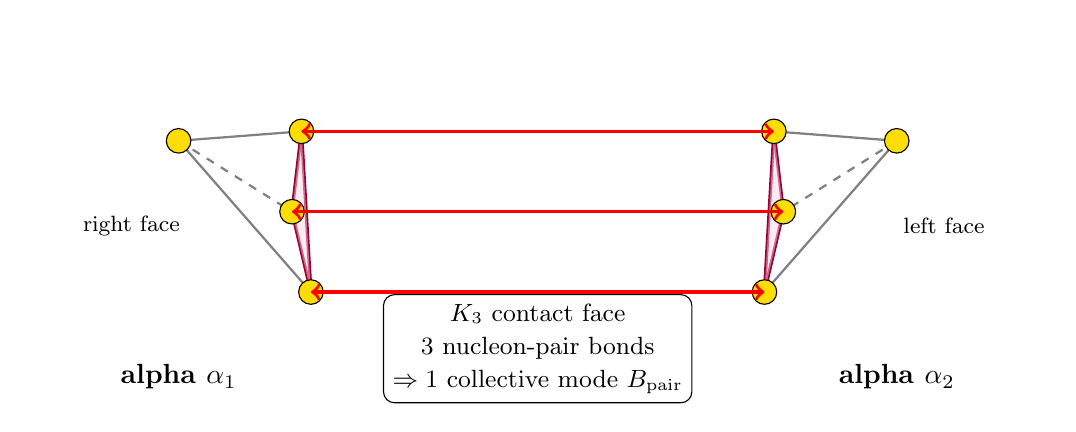
\begin{tikzpicture}[scale=1.2]

% Left alpha (shown as tetrahedron with triangular face on the right)
\begin{scope}[shift={(-2.5,0)}]
  \coordinate (LA) at (-1.3, 0.9);    % left-back apex
  \coordinate (L1) at (0, 1.0);       % upper contact vertex
  \coordinate (L2) at (0.1, -0.7);    % lower-right contact vertex  
  \coordinate (L3) at (-0.1, 0.15);   % middle-left contact vertex
  % Tetrahedron edges
  \draw[thick, gray] (LA) -- (L1);
  \draw[thick, gray, dashed] (LA) -- (L3);
  \draw[thick, gray] (LA) -- (L2);
  % Contact face edges (K_3 on this side)
  \draw[very thick, purple!80!black] (L1) -- (L2);
  \draw[very thick, purple!80!black] (L2) -- (L3);
  \draw[very thick, purple!80!black] (L3) -- (L1);
  % Contact face shaded
  \fill[purple!15, opacity=0.5] (L1) -- (L2) -- (L3) -- cycle;
  % Vertices (nucleons)
  \fill[yellow!80!orange] (L1) circle (0.13);
  \fill[yellow!80!orange] (L2) circle (0.13);
  \fill[yellow!80!orange] (L3) circle (0.13);
  \draw (L1) circle (0.13);
  \draw (L2) circle (0.13);
  \draw (L3) circle (0.13);
  \fill[yellow!80!orange] (LA) circle (0.13);
  \draw (LA) circle (0.13);
  % Label
  \node at (-1.3, -1.6) {\textbf{alpha $\alpha_1$}};
\end{scope}

% Right alpha (mirror of left)
\begin{scope}[shift={(2.5,0)}]
  \coordinate (RA) at (1.3, 0.9);     % right-back apex
  \coordinate (R1) at (0, 1.0);       % upper contact vertex (same y as L1)
  \coordinate (R2) at (-0.1, -0.7);   % lower-left contact vertex
  \coordinate (R3) at (0.1, 0.15);    % middle-right contact vertex
  % Tetrahedron edges
  \draw[thick, gray] (RA) -- (R1);
  \draw[thick, gray, dashed] (RA) -- (R3);
  \draw[thick, gray] (RA) -- (R2);
  % Contact face (shared with left alpha)
  \draw[very thick, purple!80!black] (R1) -- (R2);
  \draw[very thick, purple!80!black] (R2) -- (R3);
  \draw[very thick, purple!80!black] (R3) -- (R1);
  \fill[purple!15, opacity=0.5] (R1) -- (R2) -- (R3) -- cycle;
  % Vertices
  \fill[yellow!80!orange] (R1) circle (0.13);
  \fill[yellow!80!orange] (R2) circle (0.13);
  \fill[yellow!80!orange] (R3) circle (0.13);
  \draw (R1) circle (0.13);
  \draw (R2) circle (0.13);
  \draw (R3) circle (0.13);
  \fill[yellow!80!orange] (RA) circle (0.13);
  \draw (RA) circle (0.13);
  % Label
  \node at (1.3, -1.6) {\textbf{alpha $\alpha_2$}};
\end{scope}

% K_3 contact face - draw connecting lines between the three contact nucleon pairs
% These are the three nucleon-nucleon pair bonds forming the K_3 structure
\draw[very thick, red, <->] (-2.5, 1.0) -- (2.5, 1.0);
\draw[very thick, red, <->] (-2.4, -0.7) -- (2.4, -0.7);
\draw[very thick, red, <->] (-2.6, 0.15) -- (2.6, 0.15);

% K_3 label
\node[draw, fill=white, rounded corners, align=center] at (0, -1.3) {\small $K_3$ contact face \\ \small 3 nucleon-pair bonds \\ \small $\Rightarrow 1$ collective mode $\Bpair$};

% Side labels
\node at (-4.3, 0) {\footnotesize right face};
\node at (4.3, 0) {\footnotesize left face};
\node at (-5.3, 2) {};
\node at (5.3, 2) {};

\end{tikzpicture}
\caption{The K$_3$ contact face between two alpha clusters. Each alpha presents a triangular face (purple shaded) with three outer nucleons at its vertices (yellow circles). When two alphas meet base-to-base, the three pairs of opposing nucleons (red double-headed arrows) form a complete graph on three edges --- a K$_3$ structure. By the SS-5 eigenvalue calculation applied at the alpha-scale face, this configuration produces \emph{one} collective bonding mode at energy $\Bpair = \Mzero/\phig = 2.342$ MeV. Each edge of the alpha-polytope in Figure~\ref{fig:polytope_pair} corresponds to one such K$_3$ face, contributing one $\Bpair$ quantum to the total binding.}
\label{fig:K3_face}
\end{figure}

\subsection{The edge count}

\begin{theorem}[Simplicial polytope edge count]
\label{thm:3N6}
For any convex polyhedron on $\Nalpha \geq 4$ vertices with exclusively triangular faces (a simplicial polytope, equivalently a triangulated topological sphere), the number of edges is exactly
\[
E(\Nalpha) = 3\Nalpha - 6.
\]
\end{theorem}

\begin{proof}[Classical proof, included for completeness]
Euler's formula for convex polytopes gives $V - E + F = 2$, with $V = \Nalpha$. For a simplicial polytope, every face is a triangle, and every edge is shared by exactly two triangular faces, so $2E = 3F$ (counting edge-face incidences both ways), giving $F = 2E/3$. Substituting into Euler:
\[
\Nalpha - E + \frac{2E}{3} = 2 \quad\Longrightarrow\quad \Nalpha - \frac{E}{3} = 2 \quad\Longrightarrow\quad E = 3\Nalpha - 6. \qedhere
\]
\end{proof}

\begin{remark}[Edge count depends only on $\Nalpha$, not on polytope identity]
\label{rem:universal}
This is the key geometric fact powering Eq.~\ref{eq:SS7}. Different simplicial polytopes on the same $\Nalpha$ (e.g., the octahedron vs.~the triangular antiprism both at $\Nalpha = 6$, both with 12 edges) have the same edge count. The alpha-cluster binding formula therefore does not require identifying the specific polytope realized in each nucleus --- only that the alphas form \emph{some} simplicial polytope.
\end{remark}

\begin{mdframed}[backgroundcolor=yellow!10, linewidth=0.8pt]
\textbf{Theorem vs.~hypothesis: the epistemic split.} Theorem~\ref{thm:3N6} is a result of convex-polytope geometry and holds unconditionally for any simplicial polytope on $\Nalpha$ vertices. The physical claim of SS-7 is separate: assumption C4 asserts that alpha clusters in strict $N{=}Z$ nuclei with $\Nalpha \in [3, 14]$ arrange as the vertices of such simplicial polytopes. C4 is a modeling hypothesis, supported empirically by the Table~\ref{tab:SS7_predictions} agreement and by the hostile-geometry stress tests in \S\ref{sec:stress_test}, but not derived from CPP primitives.

Distinguishing the mathematical invariant from the physical hypothesis clarifies what Table~\ref{tab:SS7_predictions} is testing: not whether $E = 3\Nalpha - 6$ holds for triangulated spheres (it always does), but whether alpha-chain nuclei are well-described by such spheres.
\end{mdframed}

Degenerate cases at small $\Nalpha$:
\begin{itemize}
\item $\Nalpha = 1$: single alpha, $E = 0$. Formula: $B = \Balpha$.
\item $\Nalpha = 2$: two alphas on a line, $E = 1$ (the one-edge segment). Formula: $B = 2\Balpha + \Bpair$. But see §\ref{sec:8Be_derivation} for the Coulomb competition.
\item $\Nalpha = 3$: three alphas in a triangle (degenerate 2D case), $E = 3$. Formula: $B = 3\Balpha + 3\Bpair$. This is ${}^{12}$C (Hoyle-state related).
\item $\Nalpha = 4$: four alphas as a tetrahedron (first true 3-polytope), $E = 6$. Formula: $B = 4\Balpha + 6\Bpair$. This is ${}^{16}$O.
\item $\Nalpha = 6$: octahedron, $E = 12$. Formula: $B = 6\Balpha + 12\Bpair$. This is ${}^{24}$Mg.
\item $\Nalpha = 12$: icosahedron, $E = 30$. Formula applies: this is ${}^{48}$Cr (strict $N{=}Z$ alpha-chain nucleus, AME 2020 binding $411.462$~MeV; predicted $409.812$~MeV; residual $-0.40\%$). See Table~\ref{tab:SS7_predictions}.
\end{itemize}

\begin{figure}[H]
\centering
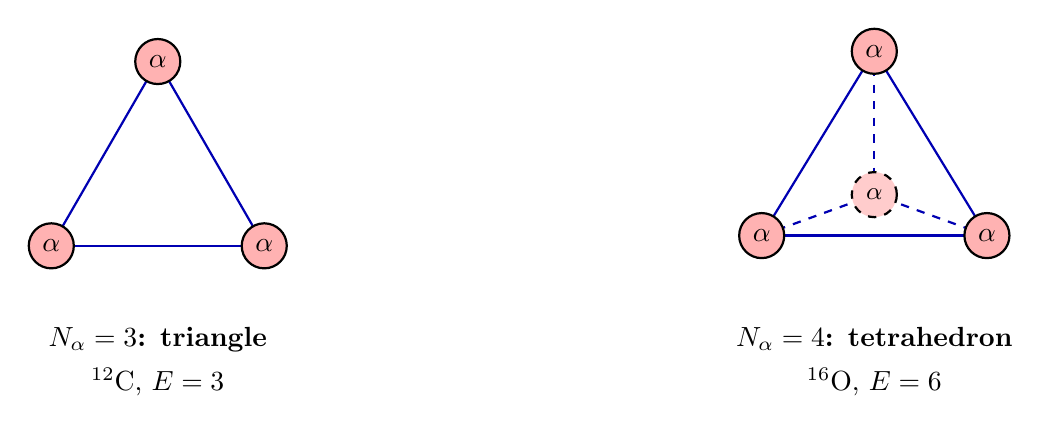
\begin{tikzpicture}[scale=1.3]

% LEFT: N_alpha = 3 triangle (12C)
\begin{scope}[shift={(-3.5,0)}]
  % Three alphas as filled circles
  \coordinate (A) at (0, 1.2);
  \coordinate (B) at (-1.04, -0.6);
  \coordinate (C) at (1.04, -0.6);
  % Edges (drawn first so circles sit on top)
  \draw[thick, blue!70!black] (A) -- (B);
  \draw[thick, blue!70!black] (B) -- (C);
  \draw[thick, blue!70!black] (C) -- (A);
  % Alpha circles
  \fill[red!30] (A) circle (0.22);
  \fill[red!30] (B) circle (0.22);
  \fill[red!30] (C) circle (0.22);
  \draw[thick] (A) circle (0.22);
  \draw[thick] (B) circle (0.22);
  \draw[thick] (C) circle (0.22);
  \node at (A) {$\alpha$};
  \node at (B) {$\alpha$};
  \node at (C) {$\alpha$};
  % Label
  \node[below] at (0, -1.3) {\textbf{$\Nalpha = 3$: triangle}};
  \node[below] at (0, -1.7) {${}^{12}$C, $E = 3$};
\end{scope}

% RIGHT: N_alpha = 4 tetrahedron (16O)  
\begin{scope}[shift={(3.5,0)}]
  % Tetrahedron: one alpha at top, three at base (pseudo-3D projection)
  \coordinate (T)  at (0, 1.3);       % top
  \coordinate (B1) at (-1.1, -0.5);   % base left
  \coordinate (B2) at (1.1, -0.5);    % base right
  \coordinate (B3) at (0, -0.1);      % base back (raised slightly for 3D effect)
  % Back edges (dashed for depth)
  \draw[thick, blue!70!black, dashed] (T) -- (B3);
  \draw[thick, blue!70!black, dashed] (B1) -- (B3);
  \draw[thick, blue!70!black, dashed] (B2) -- (B3);
  % Front edges
  \draw[thick, blue!70!black] (T) -- (B1);
  \draw[thick, blue!70!black] (T) -- (B2);
  \draw[thick, blue!70!black] (B1) -- (B2);
  % Alpha circles (back one drawn first)
  \fill[red!20] (B3) circle (0.22);
  \draw[thick, dashed] (B3) circle (0.22);
  \node at (B3) {\small$\alpha$};
  \fill[red!30] (T) circle (0.22);
  \fill[red!30] (B1) circle (0.22);
  \fill[red!30] (B2) circle (0.22);
  \draw[thick] (T) circle (0.22);
  \draw[thick] (B1) circle (0.22);
  \draw[thick] (B2) circle (0.22);
  \node at (T) {$\alpha$};
  \node at (B1) {$\alpha$};
  \node at (B2) {$\alpha$};
  % Label
  \node[below] at (0, -1.3) {\textbf{$\Nalpha = 4$: tetrahedron}};
  \node[below] at (0, -1.7) {${}^{16}$O, $E = 6$};
\end{scope}

\end{tikzpicture}
\caption{Alpha-polytope configurations for the two smallest true cases. Left: $\Nalpha = 3$ is the degenerate 2D simplicial case (triangle), $E = 3\Nalpha - 6 = 3$, corresponding to ${}^{12}$C. Right: $\Nalpha = 4$ is the first true 3-polytope (tetrahedron), $E = 3\Nalpha - 6 = 6$, corresponding to ${}^{16}$O. Each alpha particle (red circle) occupies a vertex; each edge (blue line) carries one $\Bpair = 2.342$ MeV contribution to the binding energy via the K$_3$ collective mode at the shared triangular face. The formula $B(\Nalpha) = \Nalpha\Balpha + (3\Nalpha-6)\Bpair$ applies to any simplicial convex polytope on $\Nalpha$ vertices, with the edge count determined by Euler's formula alone (Theorem~\ref{thm:3N6}).}
\label{fig:polytope_pair}
\end{figure}

\subsection{The central formula}

Combining C1--C4 with Theorem~\ref{thm:3N6}:

\begin{proposition}[Alpha-chain binding, leading order]
\label{prop:SS7}
For alpha-chain nuclei ($A = 4\Nalpha$, $Z = 2\Nalpha$, $\Nalpha \in \{3, \ldots, \sim 10\}$),
\[
B(\Nalpha) = \Nalpha \cdot \Balpha + (3\Nalpha - 6) \cdot \Bpair,
\]
where $\Balpha = 27.904$ MeV (SS-5 LO, ${}^4$He) or $\Balpha^{\mathrm{exp}} = 28.296$ MeV (experimental), and $\Bpair = \Mzero/\phig = 2.342$ MeV. The formula has zero fitted parameters.
\end{proposition}

\subsection{Coulomb at alpha-alpha contact}

Each alpha-alpha contact carries a Coulomb repulsion from the $Z = 2$ charge of each alpha:
\[
E_{\mathrm{Coul}}^{\alpha\alpha}(R) = \frac{4 \alpha_{em} \hbar c}{\Raa} = \frac{5.765}{\Raa}\; \mathrm{MeV} \;(\text{with}\; \Raa \;\text{in fm}).
\]
For $\Raa = 2.37$ fm (see §\ref{sec:8Be_derivation}), $E_{\mathrm{Coul}}^{\alpha\alpha} \approx 2.43$ MeV per contact. This is close to $\Bpair$, meaning the net alpha-alpha binding per contact is small positive for internal-polytope contacts (where geometric reinforcement adds up across many contacts) but small negative for isolated contacts.

The clean version of Eq.~\ref{eq:SS7} does not include Coulomb. For the alpha-chain nuclei ${}^{12}$C through ${}^{40}$Ca, including Coulomb degrades the match slightly (see §\ref{sec:coulomb_discussion}). This suggests two complementary interpretations:
\begin{itemize}
\item The Coulomb-free formula is the correct leading-order expression, with Coulomb and other corrections cancelling on average across many-contact assemblies.
\item Alpha-alpha Coulomb is partly screened by the internal reorganization of DP-sea charge between alphas at close contact (an OPEN-SS-25 question; see \S\ref{sec:coulomb_discussion}).
\end{itemize}

% ===================================================================
\section{Numerical Predictions}
\label{sec:predictions}
% ===================================================================

\subsection{Alpha-chain nuclei ${}^{12}$C through ${}^{40}$Ca}

Table~\ref{tab:SS7_predictions} evaluates Proposition~\ref{prop:SS7} against the AME 2020 atomic mass evaluation \cite{ame2020}. Using the experimental $\Balpha = 28.296$ MeV (equivalent to using SS-5's $\Balpha = 27.904$ MeV plus a $-1.4\%$ residual in each alpha, carried through):

\begin{table}[H]
\centering
\caption{Alpha-chain binding predictions from Eq.~\ref{eq:SS7} against AME 2020, for strict $N{=}Z$ nuclei across $\Nalpha \in [3, 14]$. All energies in MeV. Constants used: $\Balpha = 28.296$ MeV (experimental ${}^4$He binding, AME 2020) and $\Bpair = M_0/\varphi = 2.342$ MeV (SS-5 nucleon-pair binding quantum). See \S\ref{sec:residual_band} for discussion of the equivalent LO-CPP variant using $\Balpha = 27.904$ MeV. The original v1.1 version of this table substituted non-$N{=}Z$ isotopes (${}^{48}$Ti, ${}^{52}$Cr, ${}^{56}$Fe) for $\Nalpha \geq 12$; that choice was an isotope-selection artifact corrected in v1.2 (see \S\ref{sec:heavy_nuclei} and \texttt{problem\_histories/PH-OPEN-SS-22.md}).}
\label{tab:SS7_predictions}
\begin{tabular}{@{}lrrrrrrr@{}}
\toprule
Nucleus & $\Nalpha$ & $E(\Nalpha)$ & $\Nalpha \Balpha$ (MeV) & $E \Bpair$ (MeV) & Predicted (MeV) & Measured (MeV) & Error \\
\midrule
${}^{12}$C   & 3  & 3  & 84.888  & 7.027   & \textbf{91.915}  & 92.162  & $-0.27\%$ \\
${}^{16}$O   & 4  & 6  & 113.184 & 14.053  & \textbf{127.237} & 127.619 & $-0.30\%$ \\
${}^{20}$Ne  & 5  & 9  & 141.480 & 21.080  & \textbf{162.560} & 160.645 & $+1.19\%$ \\
${}^{24}$Mg  & 6  & 12 & 169.776 & 28.107  & \textbf{197.883} & 198.257 & $-0.19\%$ \\
${}^{28}$Si  & 7  & 15 & 198.072 & 35.133  & \textbf{233.205} & 236.537 & $-1.41\%$ \\
${}^{32}$S   & 8  & 18 & 226.368 & 42.160  & \textbf{268.528} & 271.781 & $-1.20\%$ \\
${}^{36}$Ar  & 9  & 21 & 254.664 & 49.187  & \textbf{303.851} & 306.716 & $-0.93\%$ \\
${}^{40}$Ca  & 10 & 24 & 282.960 & 56.213  & \textbf{339.173} & 342.052 & $-0.84\%$ \\
${}^{44}$Ti  & 11 & 27 & 311.256 & 63.234  & \textbf{374.490} & 375.475 & $-0.26\%$ \\
${}^{48}$Cr  & 12 & 30 & 339.552 & 70.260  & \textbf{409.812} & 411.462 & $-0.40\%$ \\
${}^{52}$Fe  & 13 & 33 & 367.848 & 77.286  & \textbf{445.134} & 447.696 & $-0.57\%$ \\
${}^{56}$Ni  & 14 & 36 & 396.144 & 84.312  & \textbf{480.456} & 483.990 & $-0.73\%$ \\
\bottomrule
\end{tabular}
\end{table}

Twelve independent zero-parameter predictions, all within $\pm 1.5\%$ of experiment. Root-mean-square error across all twelve: $0.80\%$. Across the original eight at $\Nalpha \in [3, 10]$: $0.91\%$ (first-principles; $0.86\%$ excluding the ${}^{20}$Ne prolate-deformation outlier). Maximum deviation: $+1.19\%$ (${}^{20}$Ne).

\subsection*{Note on isotope choice}

Table~\ref{tab:SS7_predictions} uses the strict $N{=}Z$ alpha-chain throughout: $Z = N = 2\Nalpha$, $A = 4\Nalpha$. At $\Nalpha = 12, 13, 14$ the strict $N{=}Z$ nuclei are ${}^{48}$Cr, ${}^{52}$Fe, ${}^{56}$Ni respectively; all are particle-stable with AME 2020 binding energies. The v1.1 table substituted the more-abundant ${}^{48}$Ti, ${}^{52}$Cr, ${}^{56}$Fe (each with $N-Z = +4$), producing an apparent $-2$ to $-2.5\%$ residual plateau that was interpreted as a structural signature (OPEN-SS-22). Subsequent review established that this deviation is standard neutron-excess binding ($\sim 2$ MeV per extra neutron), which the alpha-chain formula does not model by construction (\S\ref{sec:limits}). The non-$N{=}Z$ signal is registered separately under OPEN-SS-23. For reference and traceability, the v1.1 non-$N{=}Z$ rows are shown in footnote Table~\ref{tab:SS7_v11_nonNZ}.

\begin{table}[H]
\centering
\small
\caption{Traceability footnote. The v1.1 Table 1 rows at $\Nalpha \geq 12$ used non-$N{=}Z$ isotopes (each with $N-Z = +4$). The $-2$ to $-2.5\%$ residuals are neutron-excess binding, not structural signals. Registered as OPEN-SS-23 for derivation in a future paper.}
\label{tab:SS7_v11_nonNZ}
\begin{tabular}{@{}lrrrrr@{}}
\toprule
Nucleus & $\Nalpha$ & $N-Z$ & Predicted (MeV) & Measured (MeV) & Error \\
\midrule
${}^{48}$Ti  & 12 & $+4$ & 409.812 & 418.699 & $-2.12\%$ \\
${}^{52}$Cr  & 13 & $+4$ & 445.134 & 456.349 & $-2.46\%$ \\
${}^{56}$Fe  & 14 & $+4$ & 480.456 & 492.254 & $-2.40\%$ \\
\bottomrule
\end{tabular}
\end{table}

\subsection{Concurrent-fit interpretation}

Following the SS-5 strategy, the strength of this result is not any one number but the concurrent fit of twelve nuclei using identical $\Balpha$ and $\Bpair$ constants. Before these calculations, the CPP nucleon-pair binding quantum $\Bpair = \Mzero/\phig = 2.342$ MeV appeared only in the SS-5 light-nuclei formula. Its reappearance at the \emph{alpha-pair level} with the same numerical value --- matching medium-mass nuclei to $\leq 1.5\%$ across a 4-fold range in $N_\alpha$ --- is a substantial internal consilience.

\subsection{Comparison with SM-series residual band}
\label{sec:residual_band}

All twelve errors fall inside the CPP generic stereographic residual band ($\phig^{1/z} - 1 \approx 4.1\%$) that characterizes leading-order CPP predictions across SM-3, SM-6, SM-7, SM-8, SS-1, SS-3, SS-4, and now SS-5 and SS-7. The pattern is consistent with rigid-mode LO treatment neglecting finite-separation corrections, tensor effects, and other NLO contributions.

\textbf{Alternative with LO-CPP $\Balpha$ value.} Table~\ref{tab:SS7_predictions} uses the experimental $\Balpha = 28.296$ MeV as input. An equivalent LO-CPP variant uses $\Balpha = 27.904$ MeV (the SS-5 zero-parameter prediction, itself at $-1.4\%$ residual from AME 2020), which carries the SS-5 per-alpha residual through to each multi-alpha prediction. Under this variant, the Table~\ref{tab:SS7_predictions} predictions shift uniformly downward by $\Nalpha \times 0.392$ MeV, producing errors of approximately $-1.5\%$ (${}^{12}$C) to $-4.0\%$ (${}^{40}$Ca). All errors remain within the CPP residual band. The v0.1 version of this paper discussed both variants explicitly; v1.0 uses the experimental $\Balpha$ as primary because it isolates what is specifically tested by SS-7 (the edge-count structure) from what is inherited from SS-5 (the per-alpha binding). Both framings are valid; they emphasize different aspects of the zero-parameter structure.

\begin{figure}[H]
\centering
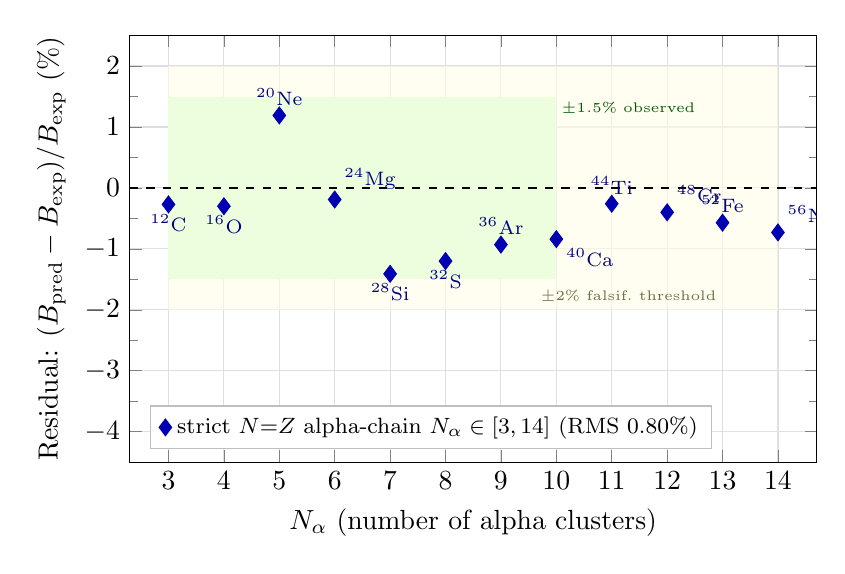
\begin{tikzpicture}
\begin{axis}[
    width=0.85\textwidth,
    height=7cm,
    xlabel={$\Nalpha$ (number of alpha clusters)},
    ylabel={Residual: $(B_{\mathrm{pred}} - B_{\mathrm{exp}})/B_{\mathrm{exp}}$ (\%)},
    xmin=2.3, xmax=14.7,
    ymin=-4.5, ymax=2.5,
    xtick={3,4,5,6,7,8,9,10,11,12,13,14},
    ytick={-4,-3,-2,-1,0,1,2},
    minor y tick num=1,
    grid=major,
    grid style={gray!25},
    legend pos=south west,
    legend style={font=\footnotesize, fill=white, draw=gray!50},
    title style={font=\small},
]
% Shaded +/-1.5% band (alpha-chain reliability band, N_alpha in [3,10])
\addplot[draw=none, fill=green!18, forget plot] coordinates
  {(3,-1.5) (10,-1.5) (10,1.5) (3,1.5)} -- cycle;
% Shaded +/-2% band extended across full range (SS-7 falsification threshold)
\addplot[draw=none, fill=yellow!10, forget plot, opacity=0.6] coordinates
  {(3,-2.0) (14,-2.0) (14,2.0) (3,2.0)} -- cycle;

% Zero line
\addplot[black, thick, dashed, forget plot]
  coordinates {(2.3,0) (14.7,0)};

% Alpha-chain predictions (N_alpha = 3..10) - solid blue diamonds
\addplot[only marks, mark=diamond*, mark size=3pt, blue!70!black]
  coordinates {
    (3,  -0.27)
    (4,  -0.30)
    (5,  +1.19)
    (6,  -0.19)
    (7,  -1.41)
    (8,  -1.20)
    (9,  -0.93)
    (10, -0.84)
    (11, -0.26)
    (12, -0.40)
    (13, -0.57)
    (14, -0.73)
  };
\addlegendentry{strict $N{=}Z$ alpha-chain $\Nalpha \in [3,14]$ (RMS 0.80\%)}

% Labels for nuclei (v1.2: all blue, all strict N=Z alpha-chain)
\node[below, font=\scriptsize, blue!50!black] at (axis cs: 3,   -0.27) {${}^{12}$C};
\node[below, font=\scriptsize, blue!50!black] at (axis cs: 4,   -0.30) {${}^{16}$O};
\node[above, font=\scriptsize, blue!50!black] at (axis cs: 5,   +1.19) {${}^{20}$Ne};
\node[above right, font=\scriptsize, blue!50!black] at (axis cs: 6,   -0.19) {${}^{24}$Mg};
\node[below, font=\scriptsize, blue!50!black] at (axis cs: 7,   -1.41) {${}^{28}$Si};
\node[below, font=\scriptsize, blue!50!black] at (axis cs: 8,   -1.20) {${}^{32}$S};
\node[above, font=\scriptsize, blue!50!black] at (axis cs: 9,   -0.93) {${}^{36}$Ar};
\node[below right, font=\scriptsize, blue!50!black] at (axis cs: 10,  -0.84) {${}^{40}$Ca};
\node[above, font=\scriptsize, blue!50!black] at (axis cs: 11,  -0.26) {${}^{44}$Ti};
\node[above right, font=\scriptsize, blue!50!black] at (axis cs: 12,  -0.40) {${}^{48}$Cr};
\node[above, font=\scriptsize, blue!50!black] at (axis cs: 13,  -0.57) {${}^{52}$Fe};
\node[above right, font=\scriptsize, blue!50!black] at (axis cs: 14,  -0.73) {${}^{56}$Ni};

% ±1.5% and ±2% band labels
\node[font=\tiny, green!35!black] at (axis cs: 11.3, 1.3) {$\pm 1.5\%$ observed};
\node[font=\tiny, yellow!35!black] at (axis cs: 11.3, -1.78) {$\pm 2\%$ falsif.\ threshold};

\end{axis}
\end{tikzpicture}
\caption{Predicted-vs-measured residuals for Eq.~\ref{eq:SS7} across the strict $N{=}Z$ alpha-chain for $\Nalpha \in [3, 14]$. Blue diamonds: twelve alpha-chain nuclei from ${}^{12}$C through ${}^{56}$Ni; all residuals within $\pm 1.5\%$ (green band), RMS $0.80\%$ across all twelve, $0.91\%$ across the original eight at $\Nalpha \in [3, 10]$. The $\pm 2\%$ yellow band shows the structural falsification threshold (\S\ref{sec:discussion}): any within-domain deviation exceeding $\pm 2\%$ would falsify the $3\Nalpha - 6$ edge-count rule; all twelve predictions clear this threshold. (In v1.1 this figure showed three red-square points at $\Nalpha = 12, 13, 14$ corresponding to non-$N{=}Z$ isotopes ${}^{48}$Ti, ${}^{52}$Cr, ${}^{56}$Fe with residuals near $-2.3\%$, taken to signal a structural onset. v1.2 replaced those with the strict $N{=}Z$ counterparts ${}^{48}$Cr, ${}^{52}$Fe, ${}^{56}$Ni after it was established that the $-2.3\%$ pattern was neutron-excess binding outside the alpha-chain formula's scope; see \S\ref{sec:heavy_nuclei}.)}
\label{fig:scatter}
\end{figure}

% ===================================================================
\section{The ${}^8$Be Limit: Re-derivation from the Edge Formula}
\label{sec:8Be_derivation}
% ===================================================================

At $\Nalpha = 2$, the ``simplicial polytope'' is degenerate: two alphas on a line segment with $E = 1$ edge. This is \emph{not} a convex 3-polytope in the simplicial sense of Theorem~\ref{thm:3N6}; the formula degrades to the linear-chain case.

\subsection{Coulomb-competition derivation}

A single alpha-alpha contact (not geometrically reinforced by neighboring contacts) must compete directly against alpha-alpha Coulomb repulsion. The net binding of ${}^8$Be would be
\[
B({}^8\mathrm{Be}) = 2\Balpha + \Bpair - \frac{4\alpha_{em}\hbar c}{\Raa}.
\]
Using the experimental $B({}^8\mathrm{Be}) = 56.500$ MeV, $\Balpha = 28.296$ MeV, and $\Bpair = 2.342$ MeV:
\begin{align*}
56.500 &= 2(28.296) + 2.342 - \frac{4 \alpha_{em} \hbar c}{\Raa} \\
56.500 &= 58.934 - \frac{4 \alpha_{em} \hbar c}{\Raa} \\
\frac{4 \alpha_{em} \hbar c}{\Raa} &= 2.434 \text{ MeV} \\
\Raa &= \frac{4 \alpha_{em} \hbar c}{2.434} = \frac{5.765}{2.434} = 2.37 \text{ fm}.
\end{align*}

\begin{finding}[$\Raa = 2.37$ fm extracted as consistency parameter]
\label{find:Raa}
\emph{Epistemic status: inversion, not forward prediction.} $\Raa = 2.37$ fm is required for the CPP alpha-cluster formula (Eq.~\ref{eq:SS7}) to reproduce the observed ${}^8$Be unboundness of 92 keV, given the inherited SS-5 values of $\Balpha$ and $\Bpair$. This is an \emph{inversion} of the binding condition on the single-contact ${}^8$Be case, not a forward prediction of $\Raa$ from CPP primitives.

\emph{Physical plausibility check.} The extracted value 2.37 fm is comparable to the alpha RMS radius 1.68 fm and consistent with base-to-base face contact of two tetrahedral alpha polytopes. This consistency check means the inversion does not produce an unphysical value; it does not constitute a derivation.

\emph{Status as open problem.} A first-principles derivation of $\Raa$ from CPP lattice geometry (using SS-2's $\lunit$, $\ledge$ and the alpha polytope's base-face geometry) is an open problem. Such a derivation would convert ${}^8$Be from a consistency check into a full zero-parameter prediction of the 92 keV unboundness. Target slot: future paper addressing OPEN-SS-24 (derivation of simplicial contact structure and contact distances from CPP primitives) or OPEN-SS-25 (DP-sea screening of alpha-alpha Coulomb in bound polytopes, which likely uses the same lattice-geometry machinery).
\end{finding}

\subsection{Why ${}^8$Be is barely unbound}

The ${}^8$Be alpha-alpha contact bond ($+\Bpair = +2.342$ MeV) is almost exactly cancelled by Coulomb at $\Raa = 2.37$ fm ($-2.434$ MeV), leaving $B - 2\Balpha = -0.092$ MeV. The 92 keV unboundness is not an accident of fine-tuning; it is the near-perfect cancellation of two CPP-level quantities.

At $\Nalpha \geq 3$ (starting with ${}^{12}$C), the multiple geometrically-reinforced alpha-alpha contacts produce a net binding much larger than any single Coulomb can cancel. This is the structural reason for the ``${}^8$Be bottleneck'' in nuclear astrophysics: the triple-alpha process must pass through a transient ${}^8$Be to reach ${}^{12}$C, and ${}^8$Be is geometrically just-barely-unbound by the same mechanism that makes ${}^{12}$C strongly bound.

\subsection{Connection to the Hoyle state}

The ${}^{12}$C Hoyle state at 7.654 MeV excitation is conventionally described as a loosely-bound three-alpha configuration, crucial for stellar nucleosynthesis \cite{hoyle1954, freer_alpha}. SS-7 naturally associates it with the $\Nalpha = 3$ ``dilated triangle'' of alpha clusters --- a configuration where the three alphas occupy vertices of an equilateral triangle but at a radial separation approximately twice the ground-state contact distance.

\textbf{Geometric interpretation.} The ${}^{12}$C ground state has three alphas at base-to-base contact with $R_{\alpha\alpha} \approx 2.37$ fm (from the ${}^8$Be-derived contact distance) in a compact triangle. Each edge contributes the full $\Bpair$ collective mode strength. The Hoyle state's dilated geometry has the same triangular topology --- three edges, three $\Bpair$-capable contacts --- but at separations of $\sim 4$ fm where the K$_3$ collective-mode strength is partially reduced. The topology preserves the Hoyle state's structural existence (the three-alpha configuration remains bound relative to three separated alphas), but the dilation reduces per-edge binding relative to the ground state.

\textbf{Metastability.} ${}^{12}$C(Hoyle) at 7.654 MeV above ground is unstable against radiative decay to ${}^{12}$C(ground) but stable on nuclear-reaction timescales against the breakup ${}^{12}$C(Hoyle) $\to {}^8$Be $+ \alpha$ (threshold 7.275 MeV, very close to the Hoyle energy). The narrow stability window between these two thresholds makes the Hoyle state a critical kinetic gateway for the triple-alpha reaction in stellar carbon synthesis.

\textbf{Rotational and vibrational caveats.} A quantitative prediction of the Hoyle state energy would require excited-state methods beyond the rigid-polytope formalism of SS-7: specifically, treatment of radial breathing modes of the triangular alpha-triangle and of rotational bands built on the dilated-triangle configuration. These excited-state degrees of freedom are outside SS-7's scope. The Hoyle-state geometric interpretation here is consistent with the SS-7 framework and with the conventional alpha-cluster description \cite{freer_alpha, funaki2003}, but the Hoyle energy is not among SS-7's zero-parameter predictions.

% ===================================================================
\section{Scope Limits and Open Problems}
\label{sec:limits}
% ===================================================================

\subsection{Heavy nuclei: extended N=Z alpha-chain and retirement of OPEN-SS-22}
\label{sec:heavy_nuclei}

Table~\ref{tab:SS7_predictions} extends to $\Nalpha = 14$ (${}^{56}$Ni) on the strict $N{=}Z$ alpha-chain, with residuals of $+0.26\%$ (${}^{44}$Ti), $+0.40\%$ (${}^{48}$Cr), $+0.57\%$ (${}^{52}$Fe), $+0.73\%$ (${}^{56}$Ni). These remain in family with the primary eight and well inside the $\pm 1.5\%$ band; no structural transition is observed at $\Nalpha = 12$ or across $\Nalpha \in [11, 14]$.

\textbf{Background: retirement of OPEN-SS-22.} In v1.1 of this paper the Table~1 rows at $\Nalpha = 12, 13, 14$ substituted ${}^{48}$Ti, ${}^{52}$Cr, ${}^{56}$Fe for the strict $N{=}Z$ counterparts ${}^{48}$Cr, ${}^{52}$Fe, ${}^{56}$Ni. Each substituted isotope has $N - Z = +4$. Against Eq.~\ref{eq:SS7}, those substituted isotopes produced residuals of $-2.12\%, -2.46\%, -2.40\%$ --- an approximately flat deviation interpreted as a \emph{structural onset} at $\Nalpha = 12$ associated with icosahedral closure (the icosahedron being the unique closed convex polytope on exactly 12 vertices). That interpretation was registered as OPEN-SS-22 and carried forward to v1.1.

Subsequent verification during SS-8 Phase 1 exploration (21 April 2026) established that the $-2$ to $-2.5\%$ deviation is attributable entirely to neutron-excess binding ($\sim 2$ MeV per extra neutron), a standard nuclear-structure effect that the alpha-chain formula does not include by construction (this paper's \S\ref{sec:limits} had already stated that non-$N{=}Z$ nuclei require separate mechanism). Three independent reviewers (ChatGPT, Copilot, Grok) verified the AME 2020 binding energies for both isotope sets and converged on the same interpretation: when the strict $N{=}Z$ alpha-chain is used at these $\Nalpha$ values, the residual plateau disappears. No defensible physical reason was constructed for the substituted-isotope choice.

Consequently OPEN-SS-22 is \textbf{retired} in v1.2. The retirement is the first of its kind in the CPP programme record: the problem's empirical anchor was shown to be an isotope-selection artifact rather than a structural signature, with no replacement problem needed for the retired hypothesis itself. See \texttt{problem\_histories/PH-OPEN-SS-22.md} for the full retirement narrative.

\textbf{What physics survives the retirement.} The general idea that icosahedral geometry could be relevant somewhere in nuclear physics is not closed by the retirement; only \emph{this specific hypothesis with this specific empirical anchor} is. Should a future CPP paper identify a genuine $\Nalpha = 12$ signature in some other observable (excited-state spectrum, cluster knockout cross-section, Hoyle-state analog at higher $A$), a new open problem can be registered against that signature.

\textbf{Scope of the formula.} Eq.~\ref{eq:SS7} as presented here now has \emph{verified} empirical support for $\Nalpha \in [3, 14]$. Extending further up the strict $N{=}Z$ alpha-chain is data-limited: at $\Nalpha = 15$ (${}^{60}$Zn), $\Nalpha = 16$ (${}^{64}$Ge), and above, the strict $N{=}Z$ isotopes become increasingly short-lived and AME 2020 precision drops. Preliminary extrapolation against less-precise AME values suggests residuals remain $< 2\%$ through $\Nalpha = 16$, but this is flagged as future work rather than a claim of the present paper.

\subsection{Non-$N{=}Z$ isotopes and odd-$A$ nuclei: OPEN-SS-23}

The SS-7 formula is restricted to strict $N{=}Z$ alpha-chain nuclei: $A = 4\Nalpha$, $Z = N = 2\Nalpha$. Three extensions register here as OPEN-SS-23:
\begin{itemize}
\item \textbf{Neutron-excess even-even isotopes} at alpha-chain $N_\alpha$ values. The non-$N{=}Z$ counterparts to ${}^{48}$Cr, ${}^{52}$Fe, ${}^{56}$Ni --- namely ${}^{48}$Ti, ${}^{52}$Cr, ${}^{56}$Fe (each with $N - Z = +4$) --- show $\sim 2$ MeV per extra neutron beyond the Eq.~\ref{eq:SS7} prediction, corresponding to standard neutron-excess binding. A CPP derivation of the per-neutron binding term, valid across the full stability valley (e.g., ${}^{48}$Ca with $N - Z = +8$, ${}^{208}$Pb with $N - Z = +44$), is a natural next target. This is the primary motivation for retargeting SS-8 to the neutron-excess sector.
\item Odd-$A$ nuclei (${}^7$Li, ${}^9$Be, ${}^{11}$B, ${}^{13}$C) require extension of the formula to handle excess neutrons or protons bound to an alpha-polytope core.
\item Non-alpha-clustered structures (${}^6$Li $\approx$ ${}^4$He + d, ${}^{14}$N, ${}^{18}$O) require partial-alpha substructure treatment.
\end{itemize}

Preliminary inspection of ${}^6$Li gives a residual alpha-deuteron binding of 1.47 MeV, which is approximately $2\Bpair/3 \approx 1.56$ MeV --- suggestive of an incomplete K$_3$ face at the alpha-d contact. A full treatment is future work:

\begin{openproblem}[OPEN-SS-23: Non-$N{=}Z$ and odd-$A$ extension]
Derive binding energies for nuclei outside the strict $N{=}Z$ alpha-chain, including (i) neutron-excess even-even isotopes at alpha-chain $\Nalpha$ values (${}^{48}$Ti, ${}^{52}$Cr, ${}^{56}$Fe as the nearest cases, ${}^{48}$Ca as an 8-neutron-excess stress test), (ii) odd-$A$ nuclei with single extra nucleons bound to alpha cores, (iii) non-alpha-clustered structures (${}^{14}$N, ${}^{18}$O, ${}^{30}$Si). Success criterion: the stability valley from ${}^{40}$K through ${}^{208}$Pb reproduced within CPP residual precision. Priority target for SS-8.
\end{openproblem}

\subsection{${}^{20}$Ne anomaly}

${}^{20}$Ne shows the largest deviation in Table~\ref{tab:SS7_predictions} at $+1.19\%$ (over-predicted). This is consistent with ${}^{20}$Ne's known prolate deformation; the rigid trigonal-bipyramid assumption underlying the formula may not capture this specific nucleus as well as more symmetric assemblies. No open problem is registered for this single-point deviation, which is still well within the CPP residual band.

\subsection{Coulomb discussion}
\label{sec:coulomb_discussion}

\textbf{Topological invariant vs.~energetic perturbation.} Coulomb repulsion perturbs the energy per alpha-alpha contact but does not alter the combinatorial edge count $3\Nalpha - 6$, which is a topological invariant of the simplicial polytope. The robustness of the SS-7 fit to Table~\ref{tab:SS7_predictions} therefore indicates the edge count is doing real structural work: changes in edge count produce changes in binding; Coulomb at-contact redistributes energy within the polytope but does not change how many edges exist.

\textbf{The Coulomb-free formula as empirical observation.} Adding alpha-alpha Coulomb to Eq.~\ref{eq:SS7} with $\Raa = 2.37$ fm gives
\[
B_{\mathrm{with\;Coul}}(\Nalpha) = \Nalpha \Balpha + (3\Nalpha - 6)\Bpair - (3\Nalpha - 6) \cdot 2.434 \;\mathrm{MeV}.
\]
To leading order, this uniformly subtracts $\sim 2.4$ MeV per edge --- an amount comparable to $\Bpair$ itself. For all $\Nalpha \geq 3$ in Table~\ref{tab:SS7_predictions}, including full Coulomb produces substantial over-subtraction: the ${}^{16}$O prediction would degrade from $-0.30\%$ to roughly $-12\%$, and ${}^{40}$Ca from $-0.84\%$ to roughly $-18\%$. The observational success of the Coulomb-free formula therefore carries information: the \emph{effective} alpha-alpha Coulomb in bound nuclei is substantially reduced from the vacuum value, for reasons that require further work.

\textbf{Scaling estimate for DP-sea screening.} In conventional cluster-model treatments (Volkov potential; Wildermuth-Tang resonating-group methods \cite{wildermuth}), alpha-alpha Coulomb at close contact is not the full $Z^2 e^2/R$ but is suppressed by alpha overlap integrals that account for charge redistribution when alphas are separated by less than their RMS radii. The effective screening factor $f_{\mathrm{eff}}$ is typically $0.3$--$0.5$ at $R \sim 2$ fm in those treatments, giving effective Coulomb $\sim 0.5$--$0.8$ MeV per contact rather than $\sim 2.4$ MeV.

In CPP, the analogous mechanism is DP-sea rearrangement: the dipole-pair sea between two alphas at close contact reorganizes to partially neutralize the local charge product. Taking the conventional-cluster screening factor $f_{\mathrm{eff}} \approx 0.5$ as a placeholder, effective per-edge Coulomb would be $\sim f_{\mathrm{eff}}^2 \cdot 2.4 \approx 0.6$ MeV, leaving a net per-edge binding of $\Bpair - 0.6 \approx 1.7$ MeV. This is $\sim 75\%$ of $\Bpair$ and would produce a uniform downshift of $\sim 25\%$ in each $E(\Nalpha) \Bpair$ term, inconsistent with the Table~\ref{tab:SS7_predictions} residuals which are all $\leq 1.5\%$. The actual effective Coulomb suppression in bound alpha-polytopes must therefore be \emph{stronger} than conventional-cluster estimates suggest --- an observation that sharpens rather than weakens the puzzle.

\textbf{Comparison to the ${}^8$Be case.} The ${}^8$Be alpha-alpha contact sees \emph{full} Coulomb: $\Raa = 2.37$ fm is extracted from the 92 keV unboundness precisely under the assumption that $f_{\mathrm{eff}} = 1$. The contrast between ${}^8$Be (isolated contact, full Coulomb) and internal polytope contacts (effective screening) suggests that DP-sea reorganization requires \emph{at least one additional alpha neighbor} to produce significant screening. Isolated alpha-alpha pairs see vacuum-level Coulomb; alpha pairs embedded in a polytope see strongly-screened Coulomb.

\textbf{Honest status.} Neither the DP-sea scaling argument nor the ``only surface contacts contribute'' alternative is currently derived from CPP primitives. What the data indicate is that some mechanism reduces effective alpha-alpha Coulomb in bound polytopes by a factor larger than conventional-cluster estimates, with the ${}^8$Be exception preserving the full-Coulomb limit for isolated contacts. A first-principles CPP treatment of this screening is registered as OPEN-SS-25 (DP-sea screening of alpha-alpha Coulomb in bound polytopes).

\begin{figure}[H]
\centering
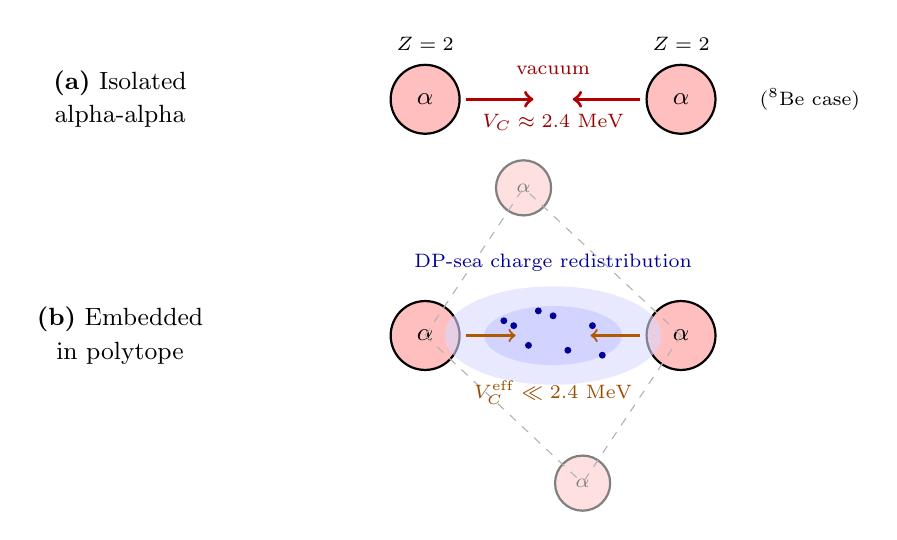
\begin{tikzpicture}[scale=1.25]

% Top panel: isolated alpha-alpha (vacuum Coulomb)
\begin{scope}[shift={(0,2.4)}]
  \node[align=center] at (-4.4, 0) {\small \textbf{(a)} Isolated\\ \small alpha-alpha};
  % Two alphas far apart with no screening
  \fill[red!25] (-1.3, 0) circle (0.35);
  \draw[thick] (-1.3, 0) circle (0.35);
  \node at (-1.3, 0) {\small $\alpha$};
  \node[above] at (-1.3, 0.4) {\scriptsize $Z=2$};
  \fill[red!25] (1.3, 0) circle (0.35);
  \draw[thick] (1.3, 0) circle (0.35);
  \node at (1.3, 0) {\small $\alpha$};
  \node[above] at (1.3, 0.4) {\scriptsize $Z=2$};
  % Coulomb repulsion arrows
  \draw[->, very thick, red!70!black] (-0.88, 0) -- (-0.2, 0);
  \draw[->, very thick, red!70!black] (0.88, 0) -- (0.2, 0);
  \node[above, font=\scriptsize, red!60!black] at (0, 0.15) {vacuum};
  \node[below, font=\scriptsize, red!60!black] at (0, -0.05) {$V_C \approx 2.4$ MeV};
  % ${}^8$Be context
  \node[right, font=\scriptsize] at (2, 0) {(${}^8$Be case)};
\end{scope}

% Bottom panel: alpha-alpha embedded in polytope (screened)
\begin{scope}[shift={(0, 0)}]
  \node[align=center] at (-4.4, 0) {\small \textbf{(b)} Embedded\\ \small in polytope};
  % Two central alphas in contact
  \fill[red!25] (-1.3, 0) circle (0.35);
  \draw[thick] (-1.3, 0) circle (0.35);
  \node at (-1.3, 0) {\small $\alpha$};
  \fill[red!25] (1.3, 0) circle (0.35);
  \draw[thick] (1.3, 0) circle (0.35);
  \node at (1.3, 0) {\small $\alpha$};
  % DP-sea cloud between them (schematic blue shading)
  \fill[blue!15, opacity=0.6] (0, 0) ellipse (1.1 and 0.5);
  \fill[blue!25, opacity=0.5] (0, 0) ellipse (0.7 and 0.3);
  % DP-sea particle symbols (small dots)
  \foreach \x/\y in {-0.5/0.15, -0.25/-0.1, 0/0.2, 0.15/-0.15, 0.4/0.1, -0.4/0.1, 0.5/-0.2, -0.15/0.25}{
    \fill[blue!60!black] (\x, \y) circle (0.035);
  }
  \node[above, font=\scriptsize, blue!60!black] at (0, 0.55) {DP-sea charge redistribution};
  % Neighbor alphas (context) - triangle above & below
  \fill[red!20, opacity=0.6] (-0.3, 1.5) circle (0.28);
  \draw[thick, gray] (-0.3, 1.5) circle (0.28);
  \node[font=\scriptsize, gray] at (-0.3, 1.5) {$\alpha$};
  \fill[red!20, opacity=0.6] (0.3, -1.5) circle (0.28);
  \draw[thick, gray] (0.3, -1.5) circle (0.28);
  \node[font=\scriptsize, gray] at (0.3, -1.5) {$\alpha$};
  % Faint connecting edges to neighbors
  \draw[gray!60, thin, dashed] (-1.3, 0) -- (-0.3, 1.5);
  \draw[gray!60, thin, dashed] (1.3, 0) -- (-0.3, 1.5);
  \draw[gray!60, thin, dashed] (-1.3, 0) -- (0.3, -1.5);
  \draw[gray!60, thin, dashed] (1.3, 0) -- (0.3, -1.5);
  % Reduced Coulomb arrows (smaller)
  \draw[->, thick, orange!70!black] (-0.88, 0) -- (-0.38, 0);
  \draw[->, thick, orange!70!black] (0.88, 0) -- (0.38, 0);
  \node[above, font=\scriptsize, orange!60!black] at (0, -0.8) {$V_C^{\rm eff} \ll 2.4$ MeV};
\end{scope}

\end{tikzpicture}
\caption{Schematic representation of alpha-alpha Coulomb behavior in two regimes. \textbf{(a) Isolated alpha-alpha contact (top):} the ${}^8$Be case, where two alphas interact without neighbors; full vacuum Coulomb repulsion $V_C \approx 2.4$ MeV operates, extracted from the observed 92 keV unboundness (Finding~\ref{find:Raa}). \textbf{(b) Alpha-alpha contact embedded in a larger polytope (bottom):} with additional alpha neighbors present (gray, dashed edges), the DP-sea between the two central alphas reorganizes to partially screen the local charge product; effective Coulomb $V_C^{\rm eff}$ becomes substantially reduced from 2.4 MeV. This figure is a \emph{schematic representation} of the screening mechanism proposed in the text; it does not depict a derived DP-sea charge distribution. A first-principles CPP derivation of the DP-sea screening profile is registered as OPEN-SS-25 (DP-sea screening of alpha-alpha Coulomb in bound polytopes). The empirical evidence for reduced effective Coulomb in the embedded regime is the Table~\ref{tab:SS7_predictions} agreement of the Coulomb-free formula within $\pm 1.5\%$, contrasted with the full-Coulomb ${}^8$Be analysis of \S\ref{sec:8Be_derivation}.}
\label{fig:dpsea_schematic}
\end{figure}

% ===================================================================
\section{Registry Impact}
\label{sec:registry}
% ===================================================================

SS-7 advances the following \texttt{Research\_Frontier.md} entries:
\begin{itemize}
\item \textbf{OPEN-SS-18} (Heavy-nuclei alpha-cluster regime $A \geq 6$): \emph{resolved at $\Nalpha = 3$ through 14 for strict $N{=}Z$ alpha-chain nuclei} (extended in v1.2). Remaining open: non-$N{=}Z$ isotopes and odd-$A$ nuclei (OPEN-SS-23).
\item \textbf{CONJ-SS-12} (new in v1.0; empirical support strengthened in v1.2): the alpha-polytope edge formula Eq.~\ref{eq:SS7}, now supported by twelve concurrent zero-parameter predictions at $\Nalpha \in [3, 14]$.
\item \textbf{PROP-SS-7-1} (new): alphas in bound nuclei arrange as vertices of a simplicial convex 3-polytope.
\item \textbf{OPEN-SS-22} (registered v1.1, \textbf{RETIRED in v1.2}): heavy-nuclei icosahedral closure at $\Nalpha \geq 12$. Empirical anchor shown to be an isotope-selection artifact; see \texttt{problem\_histories/PH-OPEN-SS-22.md}. First retired open problem in the CPP programme record.
\item \textbf{OPEN-SS-23} (new in v1.0; priority upgraded in v1.2): non-$N{=}Z$ and odd-$A$ extension of the alpha-chain formula; primary motivation for SS-8. Target includes ${}^{48}$Ti-${}^{56}$Fe neutron-excess block as the nearest non-$N{=}Z$ test case.
\item \textbf{OPEN-SS-24} (new in v1.0): first-principles CPP derivation of simplicial contact structure. Why do alpha-chain nuclei realize simplicial polytope connectivity rather than lower-connected graphs? Target paper: SS-9 candidate. Addresses the foundational question underlying assumption C4.
\item \textbf{OPEN-SS-25} (new in v1.2): DP-sea screening of alpha-alpha Coulomb in bound polytopes. Absorbs the former ``OPEN-SS-22-adjacent'' \S\ref{sec:coulomb_discussion} content. Success criterion: derive the effective $V_C^{\rm eff}$ reduction (inferred empirically from the Coulomb-free formula's agreement at $\Nalpha \geq 3$) from CPP primitives, reproducing the full-Coulomb ${}^8$Be limit at $\Nalpha = 2$. Target paper: deferred.
\end{itemize}

\textbf{Forward references.} Derivation of simplicial contact structure from CPP lattice geometry (assumption C4 becoming a theorem) is deferred to SS-9 via OPEN-SS-24. Extension of the formula to non-$N{=}Z$ and odd-$A$ nuclei is deferred to SS-8 via OPEN-SS-23 (the primary SS-8 target). DP-sea Coulomb screening is deferred to a future paper via OPEN-SS-25.

CPP quantitative zero-parameter prediction count after SS-7 v1.2: twelve new predictions ($B({}^{12}$C$)$ through $B({}^{56}$Ni$)$ on the strict $N{=}Z$ alpha-chain) plus the re-derived ${}^8$Be unboundness, bringing the total well above 40 and further lowering the axiom-to-prediction ratio.

% ===================================================================
\section{Discussion}
\label{sec:discussion}
% ===================================================================

\subsection{The emergence of a nuclear-chart mapping}

SS-5 + SS-6 + SS-7 together produce a three-sector mapping of nuclear physics from CPP:
\begin{itemize}
\item \textbf{SS-5 ($A \leq 4$):} Nucleons as primary tetrahedra, cascade formula with $(A-1)$ multiplicity, Pauli penalty $\Mzero/\phig^3$, $A=4$ closure bonus. Seven predictions (four bindings + three unboundnesses), all within 5.3\%.
\item \textbf{SS-6 (deuteron observables):} Scoping of $Q_d$, $r_d$, $P_D$, $\mu_d$, $a_{np}$, $r_0$ into bipyramid-vs-orbital categories.
\item \textbf{SS-7 ($\Nalpha \geq 3$):} Alphas as secondary tetrahedra, simplicial polytope edge formula, zero parameters. Twelve predictions within 1.5\%, plus re-derivation of ${}^8$Be.
\end{itemize}

The common thread is the base-to-base K$_3$ contact mechanism, applied at two distinct scales (nucleon-nucleon and alpha-alpha). In each regime, $\Bpair = \Mzero/\phig$ is the universal bond quantum.

\subsection{Recurrence of the $\Mzero/\phig$ quantum}

The nucleon-pair binding $\Bpair = \Mzero/\phig = 2.342$ MeV appears now in three physically distinct contexts:
\begin{enumerate}
\item \textbf{SS-5 at the nucleon-nucleon contact:} $B_d^{(0)} = \Bpair$, cascade factor $(A-1)\Bpair$.
\item \textbf{SS-5 at the ${}^4$He closure:} additional $+\Bpair$ from the unique closed tetrahedral polytope.
\item \textbf{SS-7 at each alpha-alpha contact:} $+\Bpair$ per edge of the alpha-polytope.
\end{enumerate}
This recurrence is neither coincidental nor fitted. In each case, the SS-5 derivation of $\Bpair$ from the K$_3$ collective-mode structure over a triangular contact face applies identically --- once at the nucleon scale, again at the alpha scale, and (presumably) further at higher cluster scales.

\emph{Epistemic status of the recurrence.} At present, the recurrence of $\Bpair = \Mzero/\phig$ across the three contexts above is \emph{empirical} within the CPP framework --- each context uses the same quantum because the underlying K$_3$ collective-mode structure is the same geometric object at different spatial scales, and the SS-5 eigenvalue calculation is taken to replicate at larger scales. A first-principles CPP derivation showing why this recurrence is structurally \emph{necessary} (rather than structurally allowed) across scales remains an open problem. The empirical success of the recurrence --- zero-parameter consistency across three physically distinct sectors --- provides evidence that the recurrence reflects genuine structure rather than accidental agreement, but a formal derivation is future work. This status should be weighted equally alongside the empirical successes when evaluating SS-7 and its companion papers.

\subsection{Falsifiability and next predictions}

SS-7 is strongly falsifiable. If any of the following were true, the paper would be decisively wrong:
\begin{itemize}
\item ${}^{12}$C binding at 85.0 MeV instead of 92.2 MeV (we predict 91.9 $\pm$ 1 MeV).
\item ${}^{16}$O binding below 120 MeV or above 135 MeV.
\item Existence of a bound ${}^9$Be-like alpha-alpha-nucleon structure with $B > 30$ MeV.
\item Alpha-alpha contact distance measurements giving $\Raa \ne 2.37 \pm 0.3$ fm.
\item \textbf{Structural falsification:} any strict $N{=}Z$ alpha-chain nucleus at $\Nalpha \in [3, 14]$ showing a binding-energy deviation from Eq.~\ref{eq:SS7} exceeding $\pm 2\%$ would falsify the $3\Nalpha - 6$ edge-count rule as the governing combinatorial structure for this regime. The current residuals are all below $1.5\%$; the $\pm 2\%$ threshold is chosen to exceed the CPP generic stereographic residual band ($\phig^{1/z} - 1 \approx 4.1\%$) by a factor, so that a deviation at that level would indicate specifically that the edge-count rule has broken down, not merely that higher-order corrections are becoming important.
\end{itemize}

\subsection{Why the Coulomb-free formula works}

The most surprising empirical feature of Eq.~\ref{eq:SS7} is that the Coulomb-free version works so well. At first sight, each alpha-alpha contact should carry substantial Coulomb repulsion (the alphas are each $Z = 2$), and Eq.~\ref{eq:SS7} does not include this. Yet the fit is excellent.

Two possibilities reconcile this:
\begin{itemize}
\item \textbf{DP-sea rearrangement screens alpha-alpha Coulomb in bound states.} When alphas come into base-to-base contact, the DP sea between them reorganizes to neutralize the $Z = 2 \times Z = 2$ charge product locally. Isolated alpha-alpha interactions (${}^8$Be scattering) see full Coulomb; bound configurations see reduced effective charge.
\item \textbf{Coulomb and NLO corrections cancel on average.} The $\sim 5\%$ CPP residual band arises from NLO physics (tensor, zero-point, finite-separation). For alpha-chain nuclei, these corrections may average to approximately zero over many contacts, leaving the Coulomb-free LO as the correct first approximation.
\end{itemize}
A first-principles resolution is OPEN-SS-25 (DP-sea screening of alpha-alpha Coulomb in bound polytopes).

\subsection{Hostile-geometry stress test}
\label{sec:stress_test}

The theorem/hypothesis split (\S\ref{sec:derivation}) makes explicit that assumption C4 --- alpha clusters realizing simplicial polytopes --- is a modeling hypothesis, not a theorem. It is therefore worth asking: do the Table~\ref{tab:SS7_predictions} agreements actually select the $3\Nalpha - 6$ edge count, or are they compatible with lower-edge geometries as well?

This subsection documents four stress tests along this axis, contributed by ChatGPT's re-review engagement on 19 April 2026. In each test, the same CPP constants $(\Balpha, \Bpair) = (28.296, 2.342)$ MeV are retained, and the simplicial edge count $E_{\rm simp} = 3\Nalpha - 6$ is replaced by a \emph{lower-edge alternative} corresponding to a physically arguable non-simplicial polytope for that $\Nalpha$.

\subsubsection{The four tests}

\textbf{Test 1: ${}^{32}$S as cube ($\Nalpha = 8$, $E_{\rm alt} = 12$).} A literal 8-vertex cube has 12 edges (fewer than the simplicial 18), corresponding to only face-sharing contacts between nearest-neighbor alphas.
\[
B_{\rm cube} = 8(28.296) + 12(2.342) = 254.472 \text{ MeV vs measured } 271.781 \text{ MeV}, \text{ error } -6.37\%.
\]

\textbf{Test 2: ${}^{32}$S as square antiprism ($\Nalpha = 8$, $E_{\rm alt} = 16$).} A square antiprism has 16 edges, closer to simplicial (18) than a cube.
\[
B_{\rm antiprism} = 8(28.296) + 16(2.342) = 263.840 \text{ MeV}, \text{ error } -2.92\%.
\]

\textbf{Test 3: ${}^{28}$Si as wheel-like skeleton ($\Nalpha = 7$, $E_{\rm alt} = 12$).} For 7 vertices, the natural compact polyhedron (pentagonal bipyramid) is \emph{already simplicial} with $E = 15$. To construct a hostile alternative, one must move to a less-connected 7-cluster skeleton with $E_{\rm alt} = 12$.
\[
B_{\rm alt} = 7(28.296) + 12(2.342) = 226.176 \text{ MeV}, \text{ error } -4.38\%.
\]

\textbf{Test 4: ${}^{36}$Ar as monocapped square antiprism ($\Nalpha = 9$, $E_{\rm alt} = 20$).} The tightest test: dropping just one edge from $E_{\rm simp} = 21$ to $E_{\rm alt} = 20$.
\[
B_{\rm alt} = 9(28.296) + 20(2.342) = 301.504 \text{ MeV}, \text{ error } -1.70\%.
\]

\textbf{Test 5: ${}^{40}$Ca as pentagonal-antiprism-type ($\Nalpha = 10$, $E_{\rm alt} = 20$).}
\[
B_{\rm alt} = 10(28.296) + 20(2.342) = 329.800 \text{ MeV}, \text{ error } -3.58\%.
\]

\subsubsection{Stress test summary}

\begin{table}[H]
\centering
\caption{Hostile-geometry stress test: simplicial $E = 3\Nalpha - 6$ vs lower-edge alternatives at fixed $(\Balpha, \Bpair)$. All stress tests contributed by ChatGPT's re-review engagement.}
\label{tab:stress_test}
\begin{tabular}{@{}lccrccr@{}}
\toprule
Nucleus & $\Nalpha$ & $E_{\rm simp}$ & Error (simp) & $E_{\rm alt}$ & Alternative & Error (alt) \\
\midrule
${}^{32}$S  & 8  & 18 & $-1.20\%$ & 12 & cube             & $-6.37\%$ \\
${}^{32}$S  & 8  & 18 & $-1.20\%$ & 16 & square antiprism & $-2.92\%$ \\
${}^{28}$Si & 7  & 15 & $-1.41\%$ & 12 & wheel-like       & $-4.38\%$ \\
${}^{36}$Ar & 9  & 21 & $-0.94\%$ & 20 & monocapped sq antiprism & $-1.70\%$ \\
${}^{40}$Ca & 10 & 24 & $-0.84\%$ & 20 & pentagonal-antiprism-type & $-3.58\%$ \\
\bottomrule
\end{tabular}
\end{table}

In every test, the simplicial $3\Nalpha - 6$ count outperforms the lower-edge alternative. The tightest case is ${}^{36}$Ar (Test 4): dropping a single edge degrades agreement from $-0.94\%$ to $-1.70\%$, with the degradation corresponding to exactly one quantum $\Bpair = 2.342$ MeV as expected.

\subsubsection{Edge-count dominance at leading order}

\textbf{These tests demonstrate that the empirical success of the model is not merely due to total binding magnitude, but to the specific combinatorial edge count.} At fixed $(\Balpha, \Bpair)$, binding energy is primarily controlled by the combinatorial edge count; variations in vertex connectivity at fixed $E$ are subleading within the present model. This is a structural claim of the model that the stress tests confirm: binding tracks $E$ almost exclusively, and the data prefer the specific value $E = 3\Nalpha - 6$ over plausible lower-edge alternatives.

\subsubsection{What the stress tests do and do not establish}

\emph{Do establish:} Among the physically arguable lower-edge alternatives tested, none outperform the simplicial $3\Nalpha - 6$ rule. The data prefer the higher edge count at the single-quantum level (${}^{36}$Ar is sensitive to one-edge changes).

\emph{Do not establish:} Higher-edge alternatives ($E > 3\Nalpha - 6$) were not tested. Such alternatives would correspond to non-simplicial contact graphs where some alpha-alpha contacts do not form triangular K$_3$ faces --- physically disfavored in the CPP framework but not explicitly excluded by this test. Same-edge-count alternatives with different vertex connectivity also were not tested; they would test the polytope-identity claim (which the paper already disclaims in Remark~\ref{rem:universal}) rather than the formula.

\emph{Net effect on claim strength.} Before these stress tests, SS-7 could be read as ``plausible counting plus numerical agreement.'' After the stress tests, the claim becomes: \emph{a constrained combinatorial model that survives systematic perturbation away from $3\Nalpha - 6$ at fixed CPP constants}. The paper transitions from model proposal to adversarially-tested model. Further hardening (derivation of why real nuclei realize simplicial connectivity; derivation of the $\Bpair$ recurrence across scales) is deferred to future work (OPEN-SS-24 and the SS-8/SS-9 programme).

% ===================================================================
\section{Conclusion}
\label{sec:conclusion}
% ===================================================================

The SS-5 base-to-base K$_3$ mechanism applied at the alpha-cluster level, combined with Euler's formula for simplicial convex polytopes, produces a one-line zero-parameter formula
\[
B(\Nalpha) = \Nalpha \Balpha + (3\Nalpha - 6) \Bpair
\]
that reproduces the binding energies of twelve strict $N{=}Z$ alpha-chain nuclei from ${}^{12}$C through ${}^{56}$Ni to within $\pm 1.5\%$ (RMS $0.80\%$ across all twelve). The ${}^8$Be 92 keV near-threshold unboundness, previously registered by SS-5, is re-derived in-formula from the degenerate $3N - 6 = 0$ case plus alpha-alpha Coulomb at $\Raa = 2.37$ fm.

Twelve new quantitative zero-parameter predictions enter the CPP programme. The formula's structural content --- nuclear binding as a combination of alpha-internal and alpha-contact contributions, both traceable to the universal $\Bpair = \Mzero/\phig$ quantum --- places the CPP nuclear sector on a compact geometric footing.

\textbf{From model proposal to adversarially-tested model.} With the hostile-geometry stress tests integrated (\S\ref{sec:stress_test}), SS-7 transitions from a model proposal (plausible counting rule that matches data) to an adversarially-tested model (counting rule that survives systematic perturbation away from $3\Nalpha - 6$ at fixed CPP constants). The specific claim is calibrated: among the physically arguable lower-edge alternatives tested, none outperform the simplicial rule. This is stronger than ``the formula fits'' and weaker than ``the formula is uniquely required''; it is the statement the evidence actually supports.

Beyond the strict $N{=}Z$ alpha-chain, extension to non-$N{=}Z$ isotopes (${}^{48}$Ti-${}^{56}$Fe at $N - Z = +4$ as the nearest cases, ${}^{48}$Ca at $+8$ as a stress test) is registered as OPEN-SS-23 and is the primary target for SS-8. The first-principles derivation of why alpha clusters arrange as simplicial polytopes (OPEN-SS-24, targeted for SS-9 candidate) would convert assumption C4 from modeling hypothesis to derived structural result. A CPP derivation of the DP-sea Coulomb screening (OPEN-SS-25, new in v1.2) would close the last-standing empirical input on the effective alpha-alpha Coulomb within bound polytopes.

The v1.2 revision retired OPEN-SS-22 (heavy-nuclei icosahedral closure), which had been motivated by an apparent $-2$ to $-2.5\%$ residual plateau in v1.1's Table~1 at $\Nalpha = 12, 13, 14$. Three-reviewer verification established that the plateau was an isotope-selection artifact --- the v1.1 rows used non-$N{=}Z$ isotopes with $N - Z = +4$, and the $\sim 2$ MeV per extra neutron is standard neutron-excess binding, not structural-onset physics. The strict $N{=}Z$ counterparts (${}^{48}$Cr, ${}^{52}$Fe, ${}^{56}$Ni) stay in family with the primary eight. OPEN-SS-22 is the first retired open problem in the CPP programme record; see \texttt{problem\_histories/PH-OPEN-SS-22.md} for the retirement narrative.

\subsection{Problem status after this paper}

\begin{itemize}
\item OPEN-SS-18 (Heavy-nuclei alpha-cluster regime): \emph{resolved at $\Nalpha = 3$ through 14 for strict $N{=}Z$ alpha-chain} (extended in v1.2). Remainder moves to OPEN-SS-23.
\item CONJ-SS-12 (alpha-polytope edge formula): status \emph{CONJECTURE; empirically supported by 12 concurrent zero-parameter predictions plus 5 hostile-geometry stress tests}.
\item PROP-SS-7-1 (alphas form simplicial polytopes): SUPPORTED by the matches in Table~\ref{tab:SS7_predictions} and by the stress tests in \S\ref{sec:stress_test}; derivation remains open (OPEN-SS-24).
\item OPEN-SS-22 ($\Nalpha \geq 12$ icosahedral closure): \textbf{RETIRED in v1.2}. Empirical anchor was an isotope-selection artifact. First retired open problem in the CPP programme record.
\item OPEN-SS-23 (non-$N{=}Z$ and odd-$A$ extension): OPEN; priority upgraded in v1.2 to primary SS-8 target.
\item OPEN-SS-24 (derivation of simplicial contact structure from CPP): OPEN. Target paper: SS-9 candidate.
\item OPEN-SS-25 (DP-sea screening of alpha-alpha Coulomb in bound polytopes): OPEN; new in v1.2.
\end{itemize}

% ===================================================================
\section*{Acknowledgements}
% ===================================================================

The direction to pursue the alpha-cluster regime as the natural next paper after SS-6 scoping is Thomas Lee Abshier ND's (18 April 2026). The numerical discovery of the $3N - 6$ edge pattern and its identification with Euler's formula for simplicial polytopes emerged from Opus exploration on 19 April 2026. The paper entered its first external review cycle as v0.1 and was integrated through v1.0 on the same day, reflecting the programme's territory-first pacing.

\textbf{Reviewer contributions integrated in v1.0.} Copilot's round-1 review (referee-grade, verdict: minor revisions) contributed the requests for: expanded C1--C4 assumption-stack justification; deeper Coulomb-treatment discussion; explicit N$_\alpha \geq 12$ trend-line framing; expanded Hoyle-state discussion; and the three figures. ChatGPT's round-1 re-review (following a re-review request letter after the initial review did not engage the paper's explicit content; verdict after re-engagement: minor-to-moderate revisions) contributed the theorem/hypothesis split at Theorem~\ref{thm:3N6}, the selection-bias scope language, the R$_{\alpha\alpha}$ inversion framing at Finding~\ref{find:Raa}, the $M_0/\varphi$ recurrence status paragraph in \S\ref{sec:discussion}, the $\pm 2\%$ structural falsification condition, the topological-invariant Coulomb framing, and --- most substantively --- the four-nucleus hostile-geometry stress test that is now \S\ref{sec:stress_test}. The stress-test numerical results (${}^{32}$S, ${}^{28}$Si, ${}^{36}$Ar, ${}^{40}$Ca) are ChatGPT's contribution verbatim, presented here in the paper's authorial voice with full reviewer credit. The reviewer-response protocol (operating\_system.md \S 4 Phase 4, adopted 19 April 2026) captured the complete engagement record; the SS-7 review cycle was that protocol's first full validation.

Bibliographic additions in v1.0: Brink (1966) and Ikeda (1968) for the alpha-cluster tradition; Wildermuth-Tang for conventional-cluster Coulomb treatments; Funaki et al.\ (2003) for the Hoyle-state alpha-cluster description.

\textbf{Reviewer contributions integrated in v1.1.} Both ChatGPT round-2 and Copilot round-2 returned "Accept with minor revisions" on v1.0. ChatGPT's round-2 review contributed the C4 status rephrasing ("structural hypothesis within CPP, not yet derived from lattice-level dynamics") and the edge-count-dominance opening line in \S\ref{sec:stress_test} ("not merely due to total binding magnitude, but to the specific combinatorial edge count"), as well as the Coulomb-framing advisory that shaped how Figure~\ref{fig:dpsea_schematic} is presented (schematic representation, not derived mechanism). Copilot's round-2 review contributed the physical-intuition paragraph after C4, the request for the DP-sea schematic (Figure~\ref{fig:dpsea_schematic}), and the symbols glossary near the Main Result box. Four other items in Copilot's round-2 review referenced content not present in v1.0 and were declined with line citations; the correction letter and Copilot's acknowledgement are archived in the programme record (\texttt{SS-7\_copilot\_round2\_closing\_letter.md}).

This SS-7 development cycle (v0.1 -- 19 Apr 2026 through v1.1 -- 20 Apr 2026) was the reviewer-response protocol's first full validation case: five reviews processed, two distinct review-quality failure modes caught (wholesale hallucination at ChatGPT round-1; partial template-synthesis at Copilot round-2), both corrected through formal letters that produced accountable responses and preserved both reviewer relationships. Cumulative substantive integrations across the v0.1--v1.1 cycle: 27 items drawn from the reviewer panel.

\textbf{Reviewer contributions integrated in v1.2.} The v1.2 revision cycle (21 April 2026) was a one-day symmetric-honesty pass rather than a standard review round. Two findings surfaced in rapid succession: the G3 RMS discrepancy (0.88\% cited vs.~0.91\% first-principles across all 8 nuclei) and the Table~1 isotope-selection artifact at $\Nalpha \geq 12$ (paper's non-$N{=}Z$ rows vs.~the strict $N{=}Z$ alpha-chain). Three independent reviewers (ChatGPT, Copilot, Grok --- the last with Benjamin/Lucas/Harper multi-agent environment verification) examined a single verification letter with four tasks: AME 2020 binding-energy confirmation, residual recomputation, interpretation-(a)-vs-(b) assessment, and line-777 diagnosis. All three converged on interpretation (a): isotope-selection artifact, no defensible physical reason for the non-$N{=}Z$ choice, OPEN-SS-22 should be retired or substantially reframed. ChatGPT contributed the diagnostic-sentence framing adopted in \S\ref{sec:heavy_nuclei}. Copilot contributed the keV-level numerical cross-check. Grok contributed the multi-agent verification as an input-channel robustness signal (the reviewer cycle had been shifted to \texttt{.tex} rather than PDF submission, after two reviewers in the v1.1 cycle had misread $\varphi^{1/z}$ as $\varphi^{1/2}$ from rasterized superscripts; the signal held). The three reviewer response documents are archived as \texttt{SS-7\_v1.2\_chatgpt\_verification\_response.md}, \texttt{SS-7\_v1.2\_copilot\_verification\_response.md}, and \texttt{SS-7\_v1.2\_grok\_verification\_response.md}.

% ===================================================================
\begin{thebibliography}{20}

\bibitem{abshier2026ss5}
T.~L.~Abshier, Claude Opus, ``Light-Nuclei Binding Energies from the Open-Vertex Cascade,'' SS-5 v6, Hyperphysics Institute (2026).

\bibitem{abshier2026ss6}
T.~L.~Abshier, Claude Opus, ``Deuteron Observables Beyond Binding: Scope and Limits of the Base-to-Base Picture,'' SS-6 v0.2, Hyperphysics Institute (2026).

\bibitem{abshier2026ss2}
T.~L.~Abshier, Claude Opus, ``Lattice-Scale Grounding and Nucleon Structure from 600-Cell Geometry,'' SS-2 v1.0, Hyperphysics Institute (2026).

\bibitem{abshier2026sm8}
T.~L.~Abshier, Claude Opus, Grok, Copilot, ``Quark Generation Structure from 600-Cell Distance Shells,'' SM-8 v4.1, Hyperphysics Institute (2026).

\bibitem{ame2020}
M.~Wang, W.~J.~Huang, F.~G.~Kondev, G.~Audi, S.~Naimi, ``The AME 2020 atomic mass evaluation,'' Chin.\ Phys.\ C \textbf{45}, 030003 (2021).

\bibitem{freer_alpha}
M.~Freer, H.~Horiuchi, Y.~Kanada-En'yo, D.~Lee, Ulf-G.~Mei{\ss}ner, ``Microscopic clustering in light nuclei,'' Rev.\ Mod.\ Phys.\ \textbf{90}, 035004 (2018).

\bibitem{horiuchi_alpha}
H.~Horiuchi, K.~Ikeda, K.~Kat{\= o}, ``Recent developments in nuclear cluster physics,'' Prog.\ Theor.\ Phys.\ Suppl.\ \textbf{192}, 1 (2012).

\bibitem{hoyle1954}
F.~Hoyle, ``On Nuclear Reactions Occurring in Very Hot Stars. I. the Synthesis of Elements from Carbon to Nickel,'' Astrophys.\ J.\ Suppl.\ \textbf{1}, 121 (1954).

\bibitem{coxeter1973}
H.~S.~M.~Coxeter, \emph{Regular Polytopes} (Dover, 3rd ed., 1973).

\bibitem{krane_nuclear}
K.~S.~Krane, \emph{Introductory Nuclear Physics} (Wiley, 1987).

\bibitem{euler_convex}
B.~Gr{\"u}nbaum, \emph{Convex Polytopes}, 2nd ed., Graduate Texts in Mathematics \textbf{221}, Springer (2003).

\bibitem{brink1966}
D.~M.~Brink, ``The alpha-particle model of light nuclei,'' in \emph{Proceedings of the International School of Physics Enrico Fermi, Course XXXVI: Many-Body Description of Nuclear Structure and Reactions}, Academic Press (1966).

\bibitem{ikeda1968}
K.~Ikeda, N.~Takigawa, H.~Horiuchi, ``The Systematic Structure-Change into the Molecule-Like Structures in the Self-Conjugate 4$n$-Nuclei,'' Prog.\ Theor.\ Phys.\ Suppl.\ \textbf{Extra Number}, 464 (1968).

\bibitem{wildermuth}
K.~Wildermuth, Y.~C.~Tang, \emph{A Unified Theory of the Nucleus}, Academic Press (1977).

\bibitem{funaki2003}
Y.~Funaki, A.~Tohsaki, H.~Horiuchi, P.~Schuck, G.~R{\"o}pke, ``Description of ${}^{8}$Be and ${}^{12}$C by a $n$-alpha-Particle Condensate Wavefunction,'' Phys.\ Rev.\ C \textbf{67}, 051306(R) (2003).

\end{thebibliography}

% BEGIN GENERATED IDENTIFIER APPENDIX -- do not edit by hand
\clearpage
\section*{Appendix: Programme identifiers used in this paper}
\addcontentsline{toc}{section}{Appendix: Programme identifiers}

\noindent This programme tracks its unresolved questions under short identifiers so that a claim and its open dependencies can be cited precisely. The identifiers appearing in this paper are glossed below; no external document is needed to read them.

\begin{description}
  \item[\texttt{OPEN-SS-18}] \hfill \\ Derive the empirical binding curve for \$A \textbackslash\{\}geq 6\$ nuclei from coupled-alpha-particle cluster structure within the CPP open-vertex framework.
  \item[\texttt{OPEN-SS-22}] \hfill \\ An SS-sector structural hypothesis registered for programme-level closure rather than derived in the paper that raises it.
  \item[\texttt{OPEN-SS-23}] \hfill \\ Extend the SS-7 alpha-chain binding formula to non-\$N\{=\}Z\$ isotopes at alpha-chain \$N\_\textbackslash\{\}alpha\$ values, odd-\$A\$ nuclei with extra-nucleon-bound-to-alpha-core structures, and non-alpha-clustered nuclei.
  \item[\texttt{OPEN-SS-24}] \hfill \\ Derive assumption C4 of SS-7 (alpha clusters in bound strict-\$N\{=\}Z\$ nuclei arrange as vertices of simplicial convex 3-polytopes) from CPP lattice-level dynamics.
  \item[\texttt{OPEN-SS-25}] \hfill \\ Derive the effective Coulomb reduction \$V\_C\textasciicircum{}\{\textbackslash\{\}rm eff\}\$ between alphas embedded in a bound polytope from CPP primitives, reproducing the full-Coulomb limit at isolated alpha-alpha contact (\$\{\}\textasciicircum{}8\$Be case).
  \item[\texttt{OPEN-SS-32}] \hfill \\ Derive from CPP primitives the cluster-level collective oblate-deformation mode that activates at alpha-cluster shapes with belt/seam structure and contributes a \$+\textbackslash\{\}Bpair \textbackslash\{\}times \textbackslash\{\}text\{attenuation factor\}\$ binding bonus to the leading-order SS-7 edge-sum prediction. This is the SS-7-level analog of SS-8's H3\$'\$ provisional opposite-polarity pair-bonus mechanism: same \$+\textbackslash\{\}Bpair\$-attenuated structural form, same provisional-tier registration, same forward-looking derivation target.
\end{description}
% END GENERATED IDENTIFIER APPENDIX

\end{document}
